\documentclass[times, utf8, zavrsni, numeric]{fer}
\usepackage{booktabs}
\usepackage{graphicx}
\usepackage{listings}
\usepackage{courier}
\usepackage{xcolor}
\definecolor{lightGray}{HTML}{ECECEC}
\lstset{language=Java}
\lstset{basicstyle=\footnotesize\ttfamily, tabsize=4, breaklines=true}
\lstset{backgroundcolor = \color{lightGray}, framexleftmargin=10pt, framexrightmargin=10pt}
\graphicspath{ {./slike/} }

\begin{document}

\thesisnumber{180}

\title{Generiranje notnog zapisa na temelju video zapisa vremenskih tragova
	pritisaka tipki klavira
}

\author{Ana Bagić}

\maketitle

% Ispis stranice s napomenom o umetanju izvornika rada. Uklonite naredbu \izvornik ako želite izbaciti tu stranicu.
\izvornik

% Dodavanje zahvale ili prazne stranice. Ako ne želite dodati zahvalu, naredbu ostavite radi prazne stranice.
\zahvala{}

\tableofcontents

\chapter{Uvod}
Danas je učenje sviranja raznih instrumenata puno dostupnije nego prije popularizacije Interneta. Veliku ulogu u tome imale su video streaming platforme, posebice YouTube, gdje je dostupno jako puno besplatnih video-materijala koji na razne načine pomažu zainteresiranima u svladavanju sviranja instrumenta po želji. Jedan od najpopularnijih instrumenata na YouTube-u je klavir, te je i najviše videozapisa vezano uz njega. Kako bi ga naučili svirati, studenti imaju na raspolaganju videozapise sa raznim pristupima učenju, od objašnjavanja teorije glazbe do demonstracije sviranja određene pjesme.\\

Format videozapisa koji je postao najpopularniji je upravo to demonstriranje sviranja pjesme korištenjem padajućih okomitih linija koje prikazuju u kojem trenutku je koja tipka pritisnuta. Razlog tome je što i ljudi bez velikog znanja teorije glazbe mogu naučiti svirati svoju najdražu pjesmu. Međutim, iako je broj pjesama pokriven takvim videozapisima stvarno velik, notni zapis nažalost nije uvijek dostupan, a većini glazbenika to je i dalje najjednostavniji način učenja. Ručna konverzija takvih videozapisa u notni zapis vrlo je naporna i iziskuje puno vremena. Već postoje aplikacije koje to rade za nas ali svaka od njih se oslanja isključivo na zvuk, no nisam mogla pronaći niti jednu koja to radi na temelju videozapisa.\\

Cilj ovog završnog rada je razviti aplikaciju koja iz navedenih videozapisa zna generirati notni zapis u obliku pogodnom računalu za čitanje i zapisivanje. Iz datoteke u dobivenom formatu može se, jednim od mnogih alata na Internetu, dobiti datoteka u obliku kojega ljudi znaju čitati. U okviru ovoga rada opisati ću problem generiranja notnog zapisa na temelju navedenih video-materijala. Navesti ću svoje programsko rješenje, provesti vrednovanje i objasniti rezultate, te navesti njegove dobre i loše strane.

\chapter{Opis problema}
Cilj ovog rada je omogućiti korisnicima dobivanje notnog zapisa iz video-materijala. Korisnik na nekoj video streaming platformi pronađe videozapis, u nastavku navedenog formata, čiji bi notni zapis htio dobiti i lokalno ga preuzme. Moj zadatak je razvijanje aplikacije koja na temelju odabranog videozapisa, stvori dokument s generiranim notnim zapisom u formatu koji računalo razumije. Iz datoteke koju aplikacija generira, treba biti moguće dobiti notni zapis jasan čovjeku (u npr. PDF formatu) korištenjem neke od već postojećih aplikacija na Internetu (npr. Noteflight\footnote{https://www.noteflight.com/}, MuseScore\footnote{https://musescore.com/}, Flat\footnote{https://flat.io/}).\\

U nastavku je objašnjen format ulaznog videozapisa koji se može koristiti u aplikaciji, te format izlazne datoteke koju korisnik dobije.

\section{Format videozapisa}
Izgled videozapisa iz kojega se može generirati notni zapis u mojoj aplikaciji, prikazan je na slici \ref{fig:nttdscreen}. Plavi i zeleni kvadrati predstavljaju note, odnosno tipke koje se trebaju svirati, te oni kroz vrijeme konstantno "padaju" prema klavijaturi. Kada kvadrat dođe do klavijature, pritisne se tipka koja se nalazi izravno ispod njega, te se otpusti kada kvadrat skroz "nestane" iza klavijature. Neki od videozapisa koriste tanke sive vodoravne crte kako bi označili kraj jednog takta i početak drugog, međutim te crte budu toliko blijede da se ne mogu koristiti kao pomoć kod određivanja taktova.\\

\begin{figure}[h]
	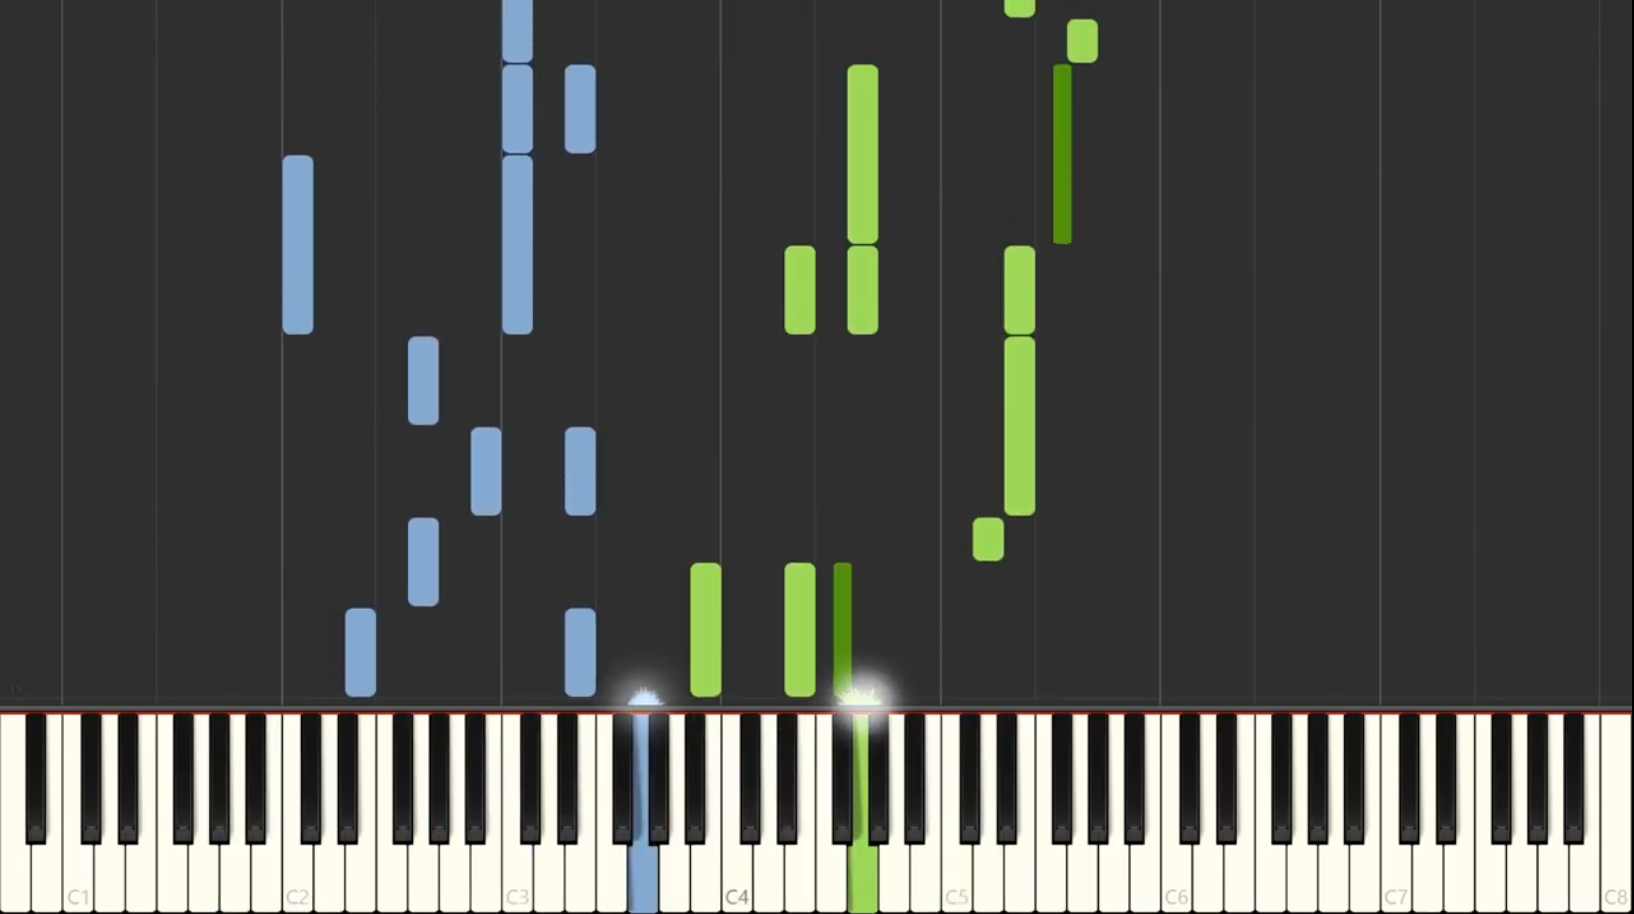
\includegraphics[scale=0.25]{nttdscreen.png}
	\centering
	\caption{Snimka zaslona korištenog videozapisa\cite{nttd}}
	\label{fig:nttdscreen}
\end{figure}

Iako se najčešće koriste plava i zelena boja za prikazivanje nota, one variraju kroz videozapise, te su zapravo stilski odabir autora. Jedino je bitno da se te dvije boje mogu razlikovati kako bi se znalo s kojom rukom se sviraju koje note. Na slici \ref{fig:nttdscreen} plava boja označava note svirane lijevom rukom, a zelena desnom. Neki autori stavljaju efekte na kvadrate (note) koji su u doticaju s klavijaturom. Iako to stvara videozapise zanimljivijima za gledatelje, otežava raspoznavanje nota mojoj aplikaciji.\\

Program koji se koristi kako bi se ovakav videozapis generirao zove se Synthesia\footnote{https://synthesiagame.com/}. Prvenstveno je namijenjena kao program za učenje sviranja klavira (klavijatura se poveže s računalom, i program prati sviranje korisnika), međutim puno je glazbenika koristi kako bi generirali ovakve videozapise, te podijelili sa Internetom svoj aranžman neke pjesme.

\section{MusicXML format}
Iz objektnog modela pjesme izgrađenog u aplikaciji, korisnik kao izlaz dobiva dokument u MusicXML formatu, kojega može iskoristiti kako bi dobio notni zapis koji mu je razumljiv.\\

MusicXML (Music Extensible Markup Language) je format datoteke baziran na XML specifikaciji. Služi za reprezentaciju zapadnjačkog notnog zapisa u obliku kojega mogu čitati i razumijeti ljudi (upoznati sa XML formatom) i računala. Izmislio ga je Michael Good, te razvio Recordare LLC - kompanija koja se bavi tehnologijom za distribuiranje glazbe i notnog zapisa na računalima, te prijenos notnog zapisa među raznim aplikacijama povezanih sa glazbom\cite{recordare}. Prva verzija MusicXML izašla je u siječnju 2004. godine\cite{musicxml}.\\

Do danas, to je postao glavni format za notni zapis na računalu, te ga koriste mnoge aplikacije koje služe za izradu, reprodukciju i dijeljenje notnog zapisa među korisnicima. Neke od njih podržavaju učitavanje datoteka u MusicXML formatu, uređivanje tog notnog zapisa, reprodukciju i izvoz u PDF, XML, MIDI, mp3 ili neki drugi format. Kroz godine njegove mogućnosti i značajke su se značajno proširile, te sada podržava većinu oznaka koje se koriste u klasičnim notnim zapisima.\\

Struktura formata slična je i drugim XML formatima, te se svaki element sastoji od oznake, nijednog, jednog ili više atributa (naziv="vrijednost"), te opcionalnog sadržaja elementa. Na slici \ref{fig:musicxml} može se vidjeti primjer MusicXML datoteke koja definira jedan takt napisan u četveročetvrtinskoj mjeri i ljestvici \textit{C-dur}. Unutar takta nalazi se jedna cijela nota.

\begin{figure}[h]
	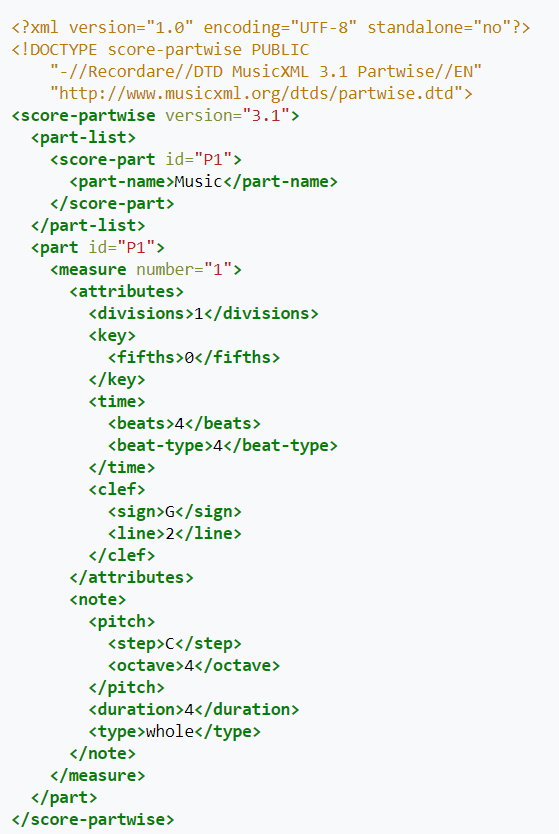
\includegraphics[scale=0.65]{musicxml.png}
	\centering
	\caption{Primjer MusicXML datoteke\cite{musicxml}}
	\label{fig:musicxml}
\end{figure}

\chapter{Korištene tehnologije}
Aplikaciju za generiranje notnog zapisa na temelju videozapisa napisala sam u programskom jeziku Java\footnote{https://www.java.com/en/} verzije 15. Za upravljanje projektom koristila sam Apache Maven\footnote{https://maven.apache.org/}. Za izgradnju korisničkog sučelja aplikacije koristila sam JavaFX\footnote{https://openjfx.io/}, a za potrebe prepoznavanja potrebnih elemenata videozapisa koristila sam OpenCV biblioteku\footnote{https://opencv.org/}.

\section{Apache Maven}
Maven je alat za automatiziranje izgradnje i upravljanja programskim projektom. Iako se najviše koristi uz programski jezik Java, može se koristiti i za projekte pisane u programskim jezicima C\#, Ruby, Scala i ostalim. Napravila ga je korporacija Apache Software Foundation, a prva verzija izašla je u srpnju 2004. godine\cite{maven}.\\

Osim automatiziranog prevođenja, testiranja i pakiranja koda, njegova najveća prednost je uvođenje ovisnosti (engl. \textit{dependencies}) prema vanjskim bibliotekama. Mogu se dodati ovisnosti prema bibliotekama iz centralnog Maven-ovog repozitorija, nekim bibliotekama treće strane (engl. \textit{third-party}) s Interneta, ili onima koje su lokalno napisane i spremljene.

\section{JavaFX}
JavaFX je biblioteka napisana za programski jezik Java koja se koristi za izgradnju korisničkog sučelja programa, a razvila ju se kompanija Oracle. Može se koristiti za razvoj desktop, web, mobilnih i ugrađenih (engl. \textit{embedded}) aplikacija. Prva verzija izašla je u prosincu 2008. godine\cite{javafx}.\\

Velika prednost JavaFX-a je ta što odvaja izradu logike aplikacije od korisničkog sučelja. Definicije vizualnih dijelova aplikacije pohranjuju se u FXML datoteke, poseban XML format, a povezivanje sa logikom aplikacije vrši se preko id-eva komponenata koje čine vizualizaciju. Kao velika pomoć dizajnerima korisničkog sučelja došao je SceneBuilder: korisničko sučelje u kojemu se kroz povuci-i-ispusti (engl. \textit{drag-and-drop}) tehniku jednostavnije slaže izgled aplikacije. JavaFX također podržava zadavanje izgleda komponenata korištenjem CSS-a.

\section{OpenCV}
OpenCV je biblioteka otvorenog koda (engl. \textit{open-source}) za računalni vid, strojno učenje i procesiranje slika i videozapisa. Razvila ju je korporacija Intel, a prva verzija izašla je u lipnju 2000. godine. Biblioteka je napisana u programskom jeziku C++, međutim do sada su napravljena sučelja (engl. \textit{API - Application Programming Interface}) koja osim C++-a podržavaju i rad u programskim jezicima Python, Java, MATLAB i JavaScript (za koji je dostupan samo podskup funkcionalnosti)\cite{opencv}. Nedostatak ove biblioteke je skoro nepostojeća dokumentacija sučelja u Javi, što mi je znatno otežalo njeno korištenje, te sam se većinom morala oslanjati na primjere sa Interneta.\\

Neke od korisnih funkcionalnosti biblioteke OpenCV koje sam koristila u izradi aplikacije su Gaussovo zamućivanje, pretvaranje slike iz BGR u HSV format, traženje rubova na slici korištenjem Canny filtera i dobivanje kontura objekata.

\subsection{Gaussovo zamućivanje}
Gaussovo zamućivanje (engl. \textit{Gaussian blur}) koristi se za smanjivanje šuma na slici. To je vrlo koristan alat u postupku prepoznavanja objekata na slici, jer zaglađuje nagle promijene u intenzitetu piksela, a većinu slike i dalje ostavlja nepromijenjenom i objekte na njoj prepoznatljivim. Rezultat primjene filtera može se vidjeti na slici \ref{fig:gblur}.\\

Algoritam se primjenjuje na svaki piksel slike. Npr. za piksel označen crvenom bojom na slici \ref{fig:gblur}, gleda se sivi pravokutnik oko njega koji se naziva jezgra (engl. \textit{kernel}). Ona je u ovom slučaju dimenzija 7x7, no one mogu biti i drugačije ovisno o efektu koji se želi postići (veća jezgra - veće zaglađivanje slike) ali trebaju biti neparni brojevi kako bi piksel mogao biti centriran unutar jezgre.

\begin{figure}[h]
	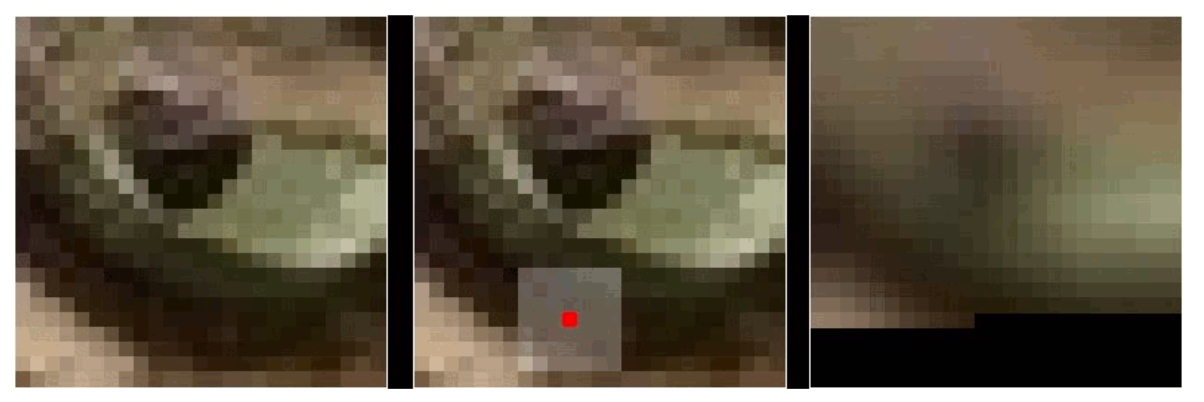
\includegraphics[scale=0.5]{gblur.png}
	\centering
	\caption{Primjer Gaussian blur filtera\cite{gauss}}
	\label{fig:gblur}
\end{figure}

Kako bi se izračunala nova vrijednost piksela, računa se težinska prosječna vrijednost svih piksela unutar jezgre. Baš kao i kod Gaussove krivulje, pikseli bliže centru jezgre imati će veću težinu, a oni dalje manju. Zadavanjem veće standardne devijacije, razlike u težini piksela bliže i dalje centru jezgre biti će manje, a manjom devijacijom dobivamo veću razliku, tj. vrh krivulje biti će izraženiji, a pikseli bliže centru imati će puno veću težinu\cite{gauss}.\\

Ovdje se može vidjeti primjer korištenja Gaussovog zamućivanja s bibliotekom OpenCV. Koristi se jezgra veličine 3x3, a iznos standardne devijacije iznosi 5.
\begin{lstlisting}
Imgproc.GaussianBlur(srcFrame, destFrame, new Size(3, 3), 5);
\end{lstlisting}

\subsection{Pretvaranje slike iz BGR u HSV prostor boja}
Prostor boja je način na koji se predstavljaju boje prisutne u slici, a koje daju slici tu određenu nijansu. Pretpostavljeni prostor boja u OpenCV-u je BGR (Blue, Green, Red), kod kojega različiti intenziteti plave, zelene i crvene boje daju različite nijanse boja\cite{colore}. Prikaz BGR prostora boja može se vidjeti na slici \ref{fig:bgr}.\\

Prostor boja koji je pogodan za prepoznavanje obruba elemenata slike je HSV (Hue, Saturation, Value), koji je definiran na sličan način kako ljudi percipiraju boju. Hue predstavlja boju u osnovnom smislu te riječi, a vrijednosti idu od 0 do 360 stupnjeva, međutim u OpenCV-u one se prikazuju u rasponu 0-179. Saturation predstavlja zasićenje boje odnosno količinu sive boje, gdje vrijednosti u OpenCV-u idu od 0 (najviše sive) do 255 (najzasićenija boja). Value opisuje svjetlinu, tj. intenzitet boje, a vrijednosti se nalaze u rasponu od 0 (potpuno crno) do 255 (najsvjetlije)\cite{colorh}. Prikaz HSV prostora boja može se vidjeti na slici \ref{fig:hsv}.

\begin{figure}[h]
	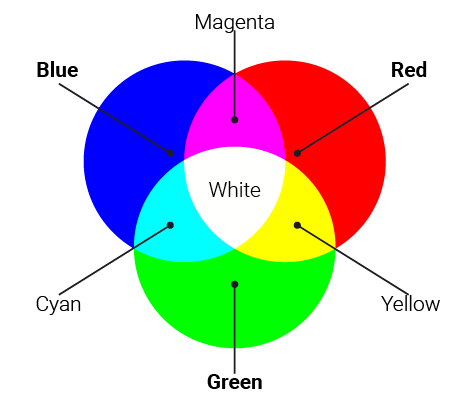
\includegraphics[scale=0.55]{bgr.png}
	\centering
	\caption{BGR prostor boja\cite{rgb}}
	\label{fig:bgr}
\end{figure}

\begin{figure}[h]
	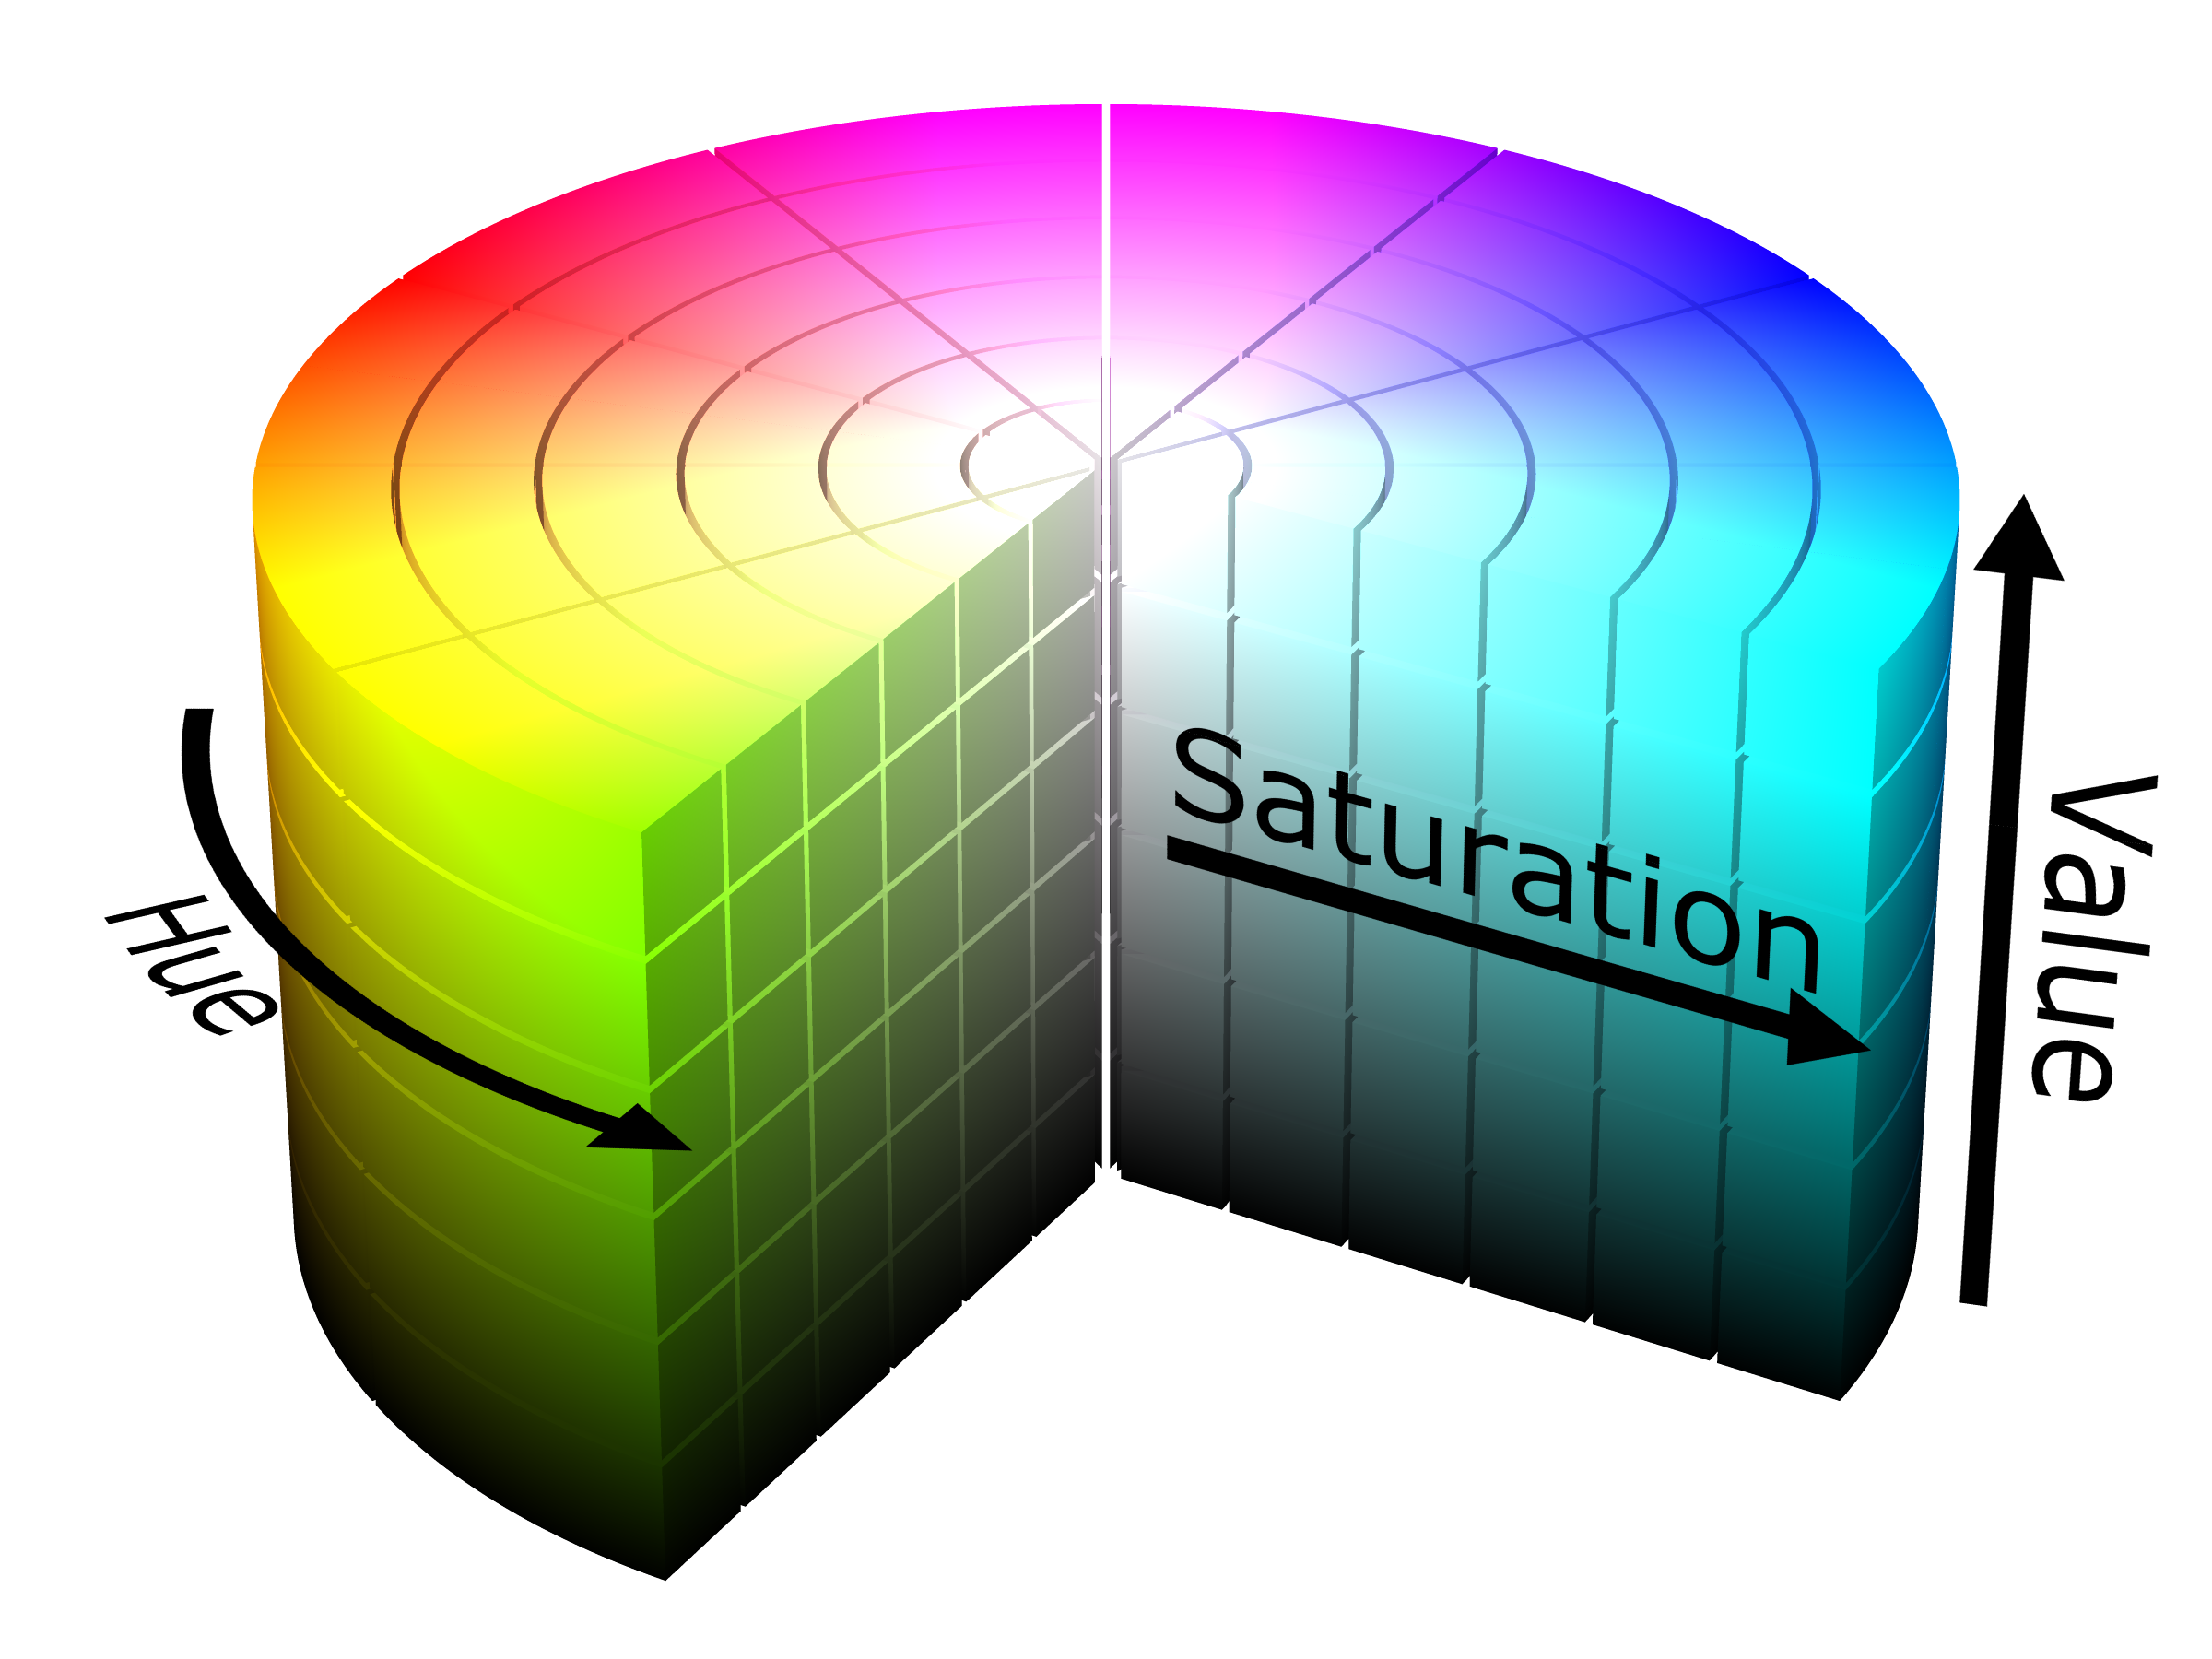
\includegraphics[scale=0.11]{hsv.png}
	\centering
	\caption{HSV prostor boja\cite{hsv}}
	\label{fig:hsv}
\end{figure}

OpenCV nudi mnoge metode konverzije iz jednog prostora boja u drugi, a meni je najzanimljiviji bio onaj koji pretvara BGR u HSV. Nad svakim pikselom u BGR prostoru boja provodi se jednostavna aritmetika kako bi se dobila HSV vrijednost piksela.

\subsection{Cannyev detektor rubova}
Cannyev detektor rubova je algoritam kojeg je razvio John F. Canny 1986. godine, a služi prepoznavanju rubova objekata na slici, kako bi se mogli odrediti njihovi položaji. Rubovi su zapravo nagle promjene u intenzitetu susjednih piksela. Ispravan algoritam za detekciju rubova bi trebao ispravno odrediti što više rubova prisutnih na slici, ispravno pronaći centar ruba i ne bi smio pronalaziti nepostojeće rubove\cite{canny1}.\\

Cannyev filter radi u 4 koraka: smanjivanje šuma slike korištenjem Gaussovog zamućenja, računanje intenziteta gradijenata, stanjivanje rubova na jedan piksel brisanjem piksela koji nisu maksimalni i na kraju uspoređivanje vrijednosti piksela pronađenih rubova s gornjim i donjim pragom, kako bi se odredilo treba li ih odbaciti ili zadržati. Sve gradijente veće od gornjeg praga se prihvaća kao rub, a sve manje od donjeg praga se odbacuje. U slučaju da je gradijent između dva praga, prihvaća se ako piksel dodiruje neki drugi koji ima gradijent veći od gornjeg praga.\\

Na slici \ref{fig:canny} može se vidjeti rezultat primjene Cannyevog filtera. Prva slika je originalna, druga je slika nakon primjene Sobel jezgre za pronalazak intenziteta gradijenata, a treća je konačan rezultat. OpenCV koristi Gaussovo zamućenje sa 5x5 jezgrom i standardnom devijacijom 1, i 3x3 Sobel jezgru za pronalazak intenziteta gradijenata\cite{canny2}.

\begin{figure}[h]
	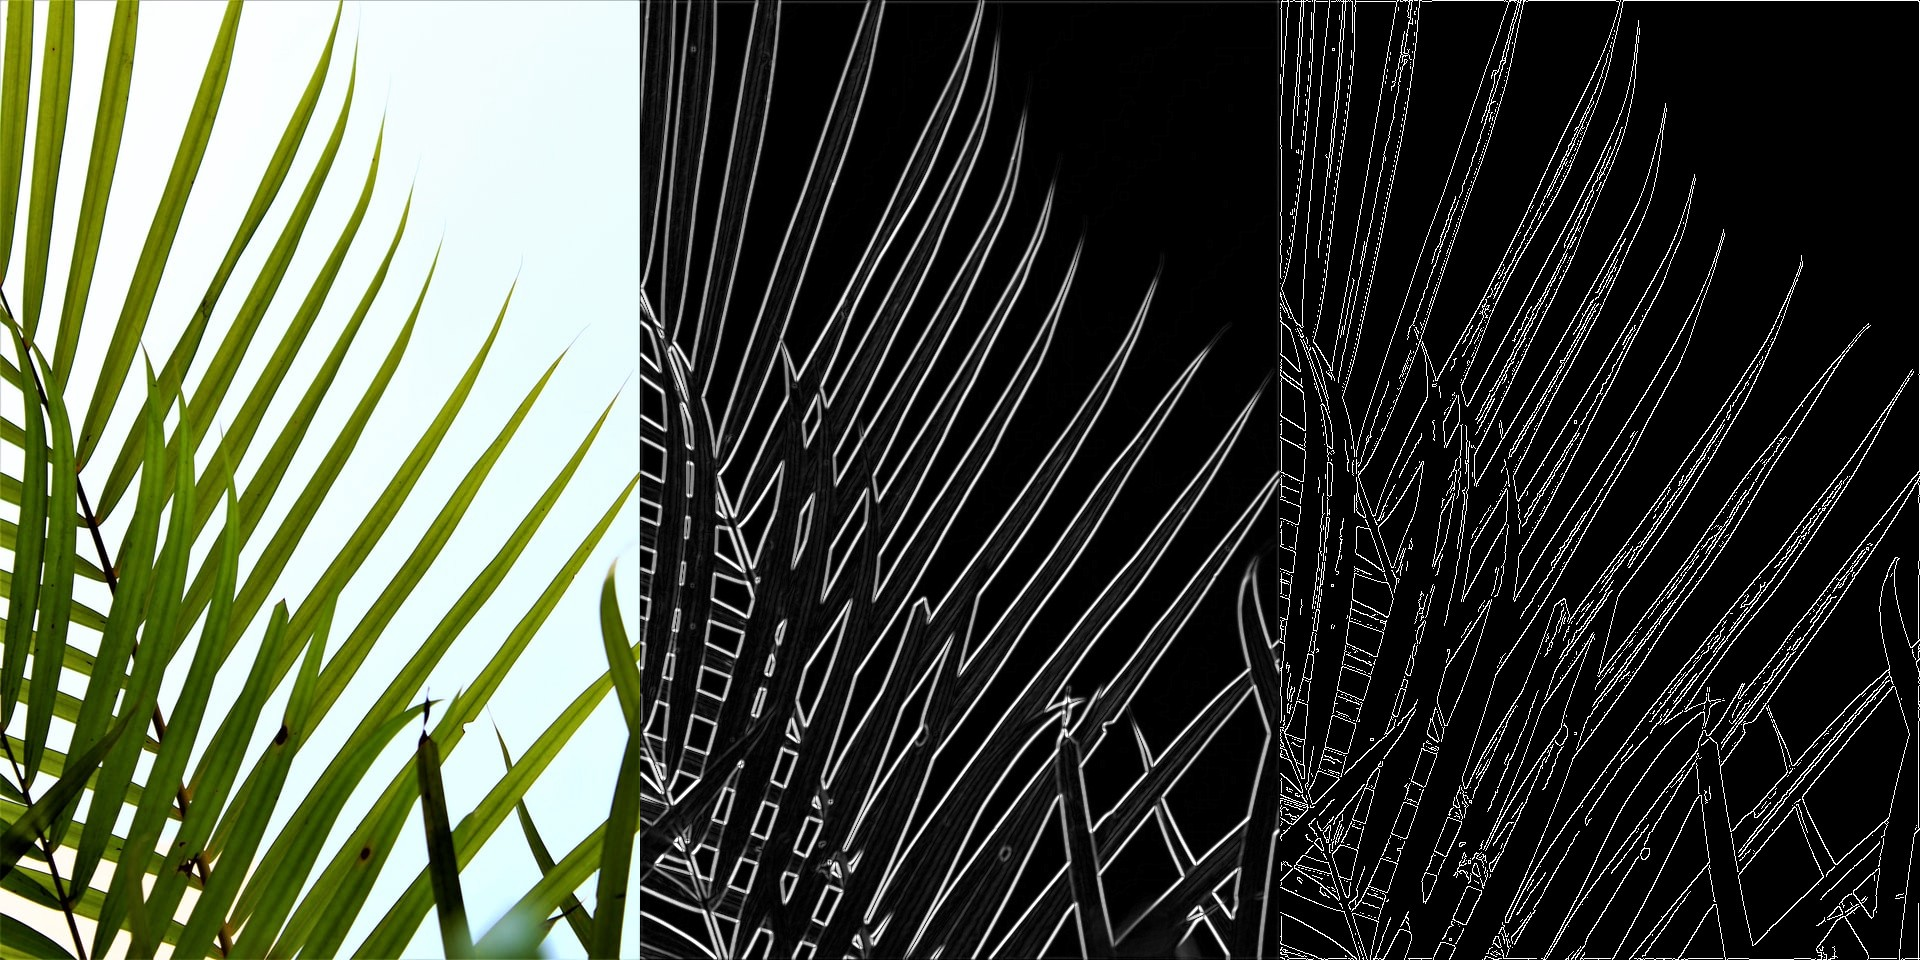
\includegraphics[scale=0.22]{canny.jpeg}
	\centering
	\caption{Primjer primjene Cannyevog filtera\cite{canny2}}
	\label{fig:canny}
\end{figure}

\subsection{Dobivanje pravokutnika koji obrubljuju konture}
Konture se definiraju kao linije koje spajaju sve točke s istim intenzitetom. Upravo zato, prije pronalaska kontura, pametno je pretvoriti sliku u binarni oblik (npr. Cannyevim filterom). Algoritam pronalaska kontura iz rubova elemenata slike gradi te linije, odnosno skup točaka, te kao rezultat vraća skup tih linija - kontura. Pravokutnici koji obrubljuju konture (engl. \textit{bounding rectangles}), dobivaju se tako da se odrede minimalne i maksimalne x i y koordinate unutar kojih se nalaze sve točke kontura. Na slici \ref{fig:bounding} mogu se vidjeti ravan (zeleni) i rotiran (crveni) obrubljujući pravokutnik.

\begin{figure}[h]
	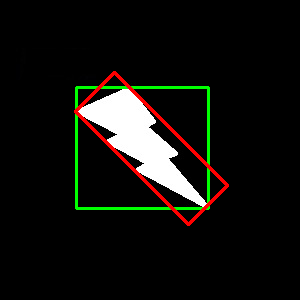
\includegraphics[scale=0.5]{bounding.png}
	\centering
	\caption{Primjer obrubljujućih pravokutnika\cite{bounding}}
	\label{fig:bounding}
\end{figure}

\chapter{Implementacija programa}
Cijeli tijek rada moje aplikacije mogu podijeliti u 4 glavna dijela. Podijelila sam ih tako kako bih smanjila međuovisnost između glavnih komponenata aplikacije, te olakšala testiranje rada svakog od dijelova. Aplikacija na početku traži informacije od korisnika, zatim provodi algoritam prepoznavanja nota iz videozapisa, nakon toga traži tonalitet, tempo i ritam pjesme, te se prilagođava note njima i na kraju dobiven model pjesme formatira u MusicXML datoteku.

\section{Dobivanje informacija od korisnika}
Pri pokretanju aplikacije, od korisnika se zatraži da upiše ime i izvođača pjesme. U slučaju da korisnik ostavi prazno neka od tih mjesta, aplikacija kod izgradnje konačne datoteke postavlja njihove vrijednosti na "Pjesma" i "Autor". Korisnika se također pita da na disku pronađe videozapis iz kojega želi generirati notni zapis, vidi sliku \ref{fig:screen1}.

\begin{figure}[h]
	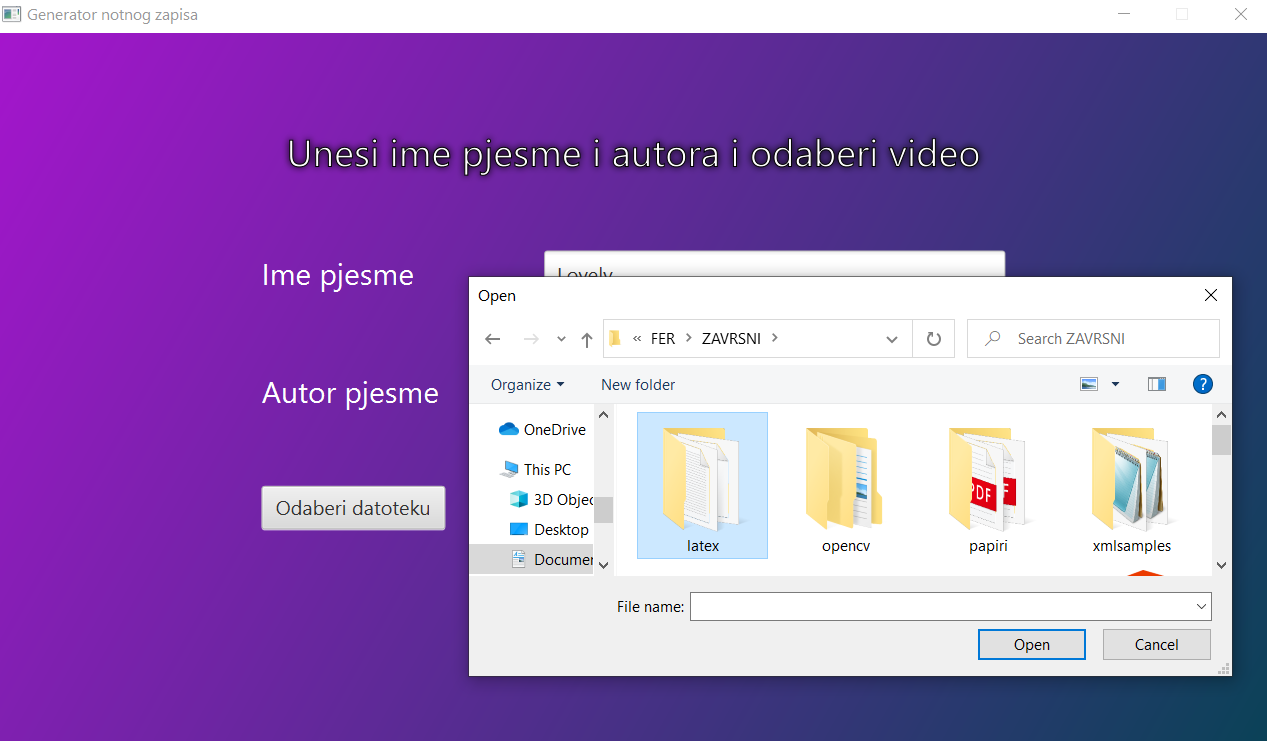
\includegraphics[scale=0.43]{screen1.png}
	\centering
	\caption{Snimka zaslona za odabir pjesme}
	\label{fig:screen1}
\end{figure}

Iako se najčešće u ovakvim videozapisima javlja puna klavijatura sa 88 tipki (7 i pol oktava) koja se nalazi na klasičnim koncertnim klavirima, nije uvijek tako. Neki od videozapisa, pogotovo oni namijenjeni početnicima, prikazuju samo dio pune klavijature, najčešće 3 do 5 oktava. Iz toga razloga se od korisnika traži da odabere jednu od ponuđenih raspona klavijatura. Nadogradnja aplikacije s novim klavijaturama je vrlo jednostavna. Napiše se novi razred koji se izvede iz razreda \textit{Keyboard} te se implementiraju sljedeće metode:

\begin{lstlisting}
int getWhiteKeys();				int getRealOctave(int octave);
double getOffset();				String getRange();
\end{lstlisting}

Također se u datoteku \textit{config\textbackslash keyboards.txt} doda puno ime paketa i razreda klavijature (engl. \textit{fqcn}) kako bi se razredi mogli učitati. Dodavanjem klavijature na taj način, kod idućeg pokretanja vidjeti će se u izborniku. Dinamičko učitavanje razreda postigla sam koristeći generičku tvornicu na sljedeći način:

\begin{lstlisting}
List<String> keyboardFQCN = Files.lines(Paths.get(Constants.PATH_TO_KEYBOARDS)).collect(Collectors.toList());

for(String k : keyboardFQCN) {
	Class<Keyboard> keyboard = (Class<Keyboard>)Class.forName(k);
	keyboards.add(keyboard.getConstructor().newInstance());
}
\end{lstlisting}

Od korisnika tražim da upiše i mjeru u kojoj se nalazi pjesma te tempo pjesme, tj. broj otkucaja u minuti (engl. \textit{beats per minute}). Određivanje toga iz videozapisa mi se činilo izrazito komplicirano (ako ne i nemoguće s mojim trenutnim znanjem u računarstvu i teoriji glazbe). Npr. razlika između pjesme u mjeri 2/4 i 4/4 je vrlo mala, a većinom se određuje po sluhu, kao i između mjere 3/4 i 6/8. Takvi parametri su često rezultat slobode glazbenika, te ih je vrlo teško deterministički odrediti. Slična stvar vrijedi i za tempo. Mogu odrediti da postoji nota koja traje x i ona koja traje 2x, ali problem je što tempo može biti 60bpm, a može biti i 120bpm, pa se ne može odrediti je li x polovinka, četvrtinka, osminka ili nešto četvrto. Ne pomaže niti frekvencijska analiza pojavljivanja duljina nota. Uzmimo za primjer pjesmu u kojoj je jedinica mjere četvrtinka. To ne mora značiti da će najviše zastupljena i biti četvrtinka, jer postoje pjesme u kojima ima najviše i šesnaestinki, i osminki i polovinki. Međutim, tempo koji je korisnik unio promatram samo kao orijentir prema stvarnom tempu (objašnjeno u nastavku). Zaslon za odabir ovih parametara može se vidjeti na slici \ref{fig:screen2}.

\begin{figure}[h]
	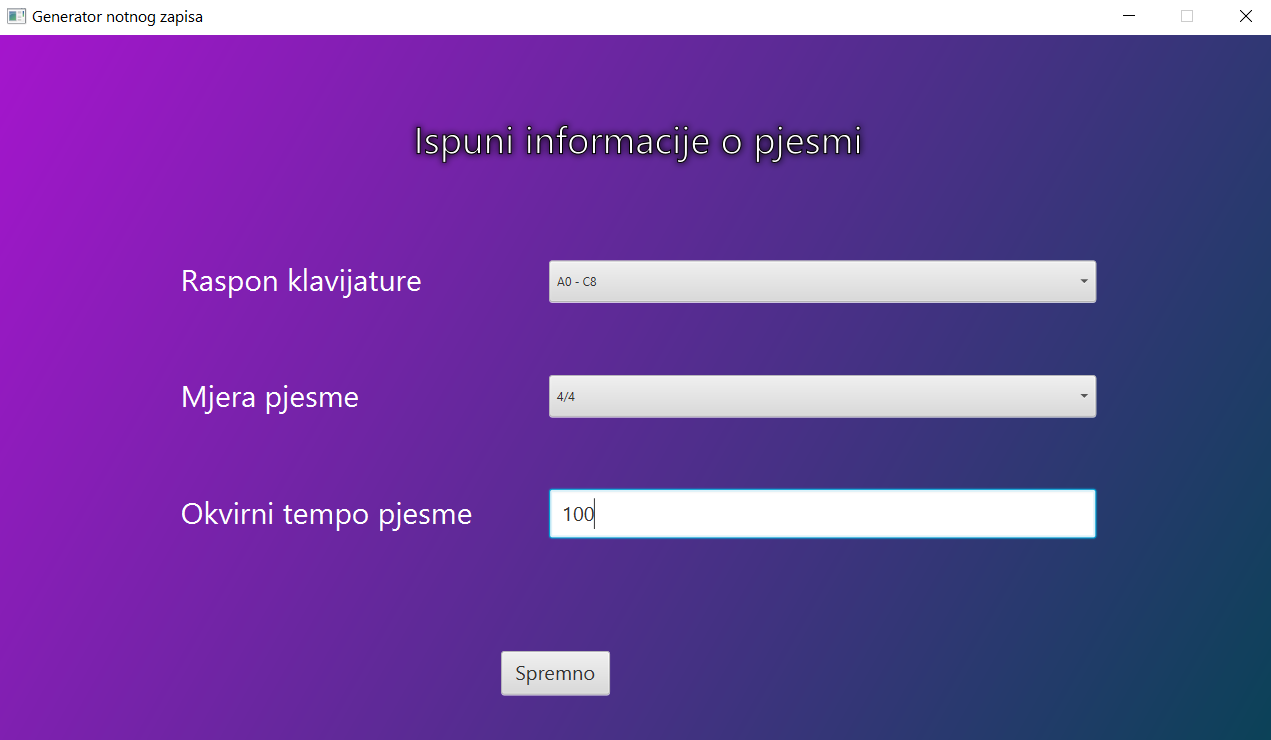
\includegraphics[scale=0.43]{screen2.png}
	\centering
	\caption{Snimka zaslona za određivanje parametara pjesme}
	\label{fig:screen2}
\end{figure}

\subsection{Određivanje područja s notama}
Neki videozapisi nemaju prikazanu klavijaturu i područje s notama na cijeloj površini videozapisa. Moguće je da imaju okvir sa dodatnim informacijama za korisnika koje su nepotrebne (i smetaju) u procesu generiranja notnog zapisa, vidi sliku \ref{fig:milreasons}.

\begin{figure}[h]
	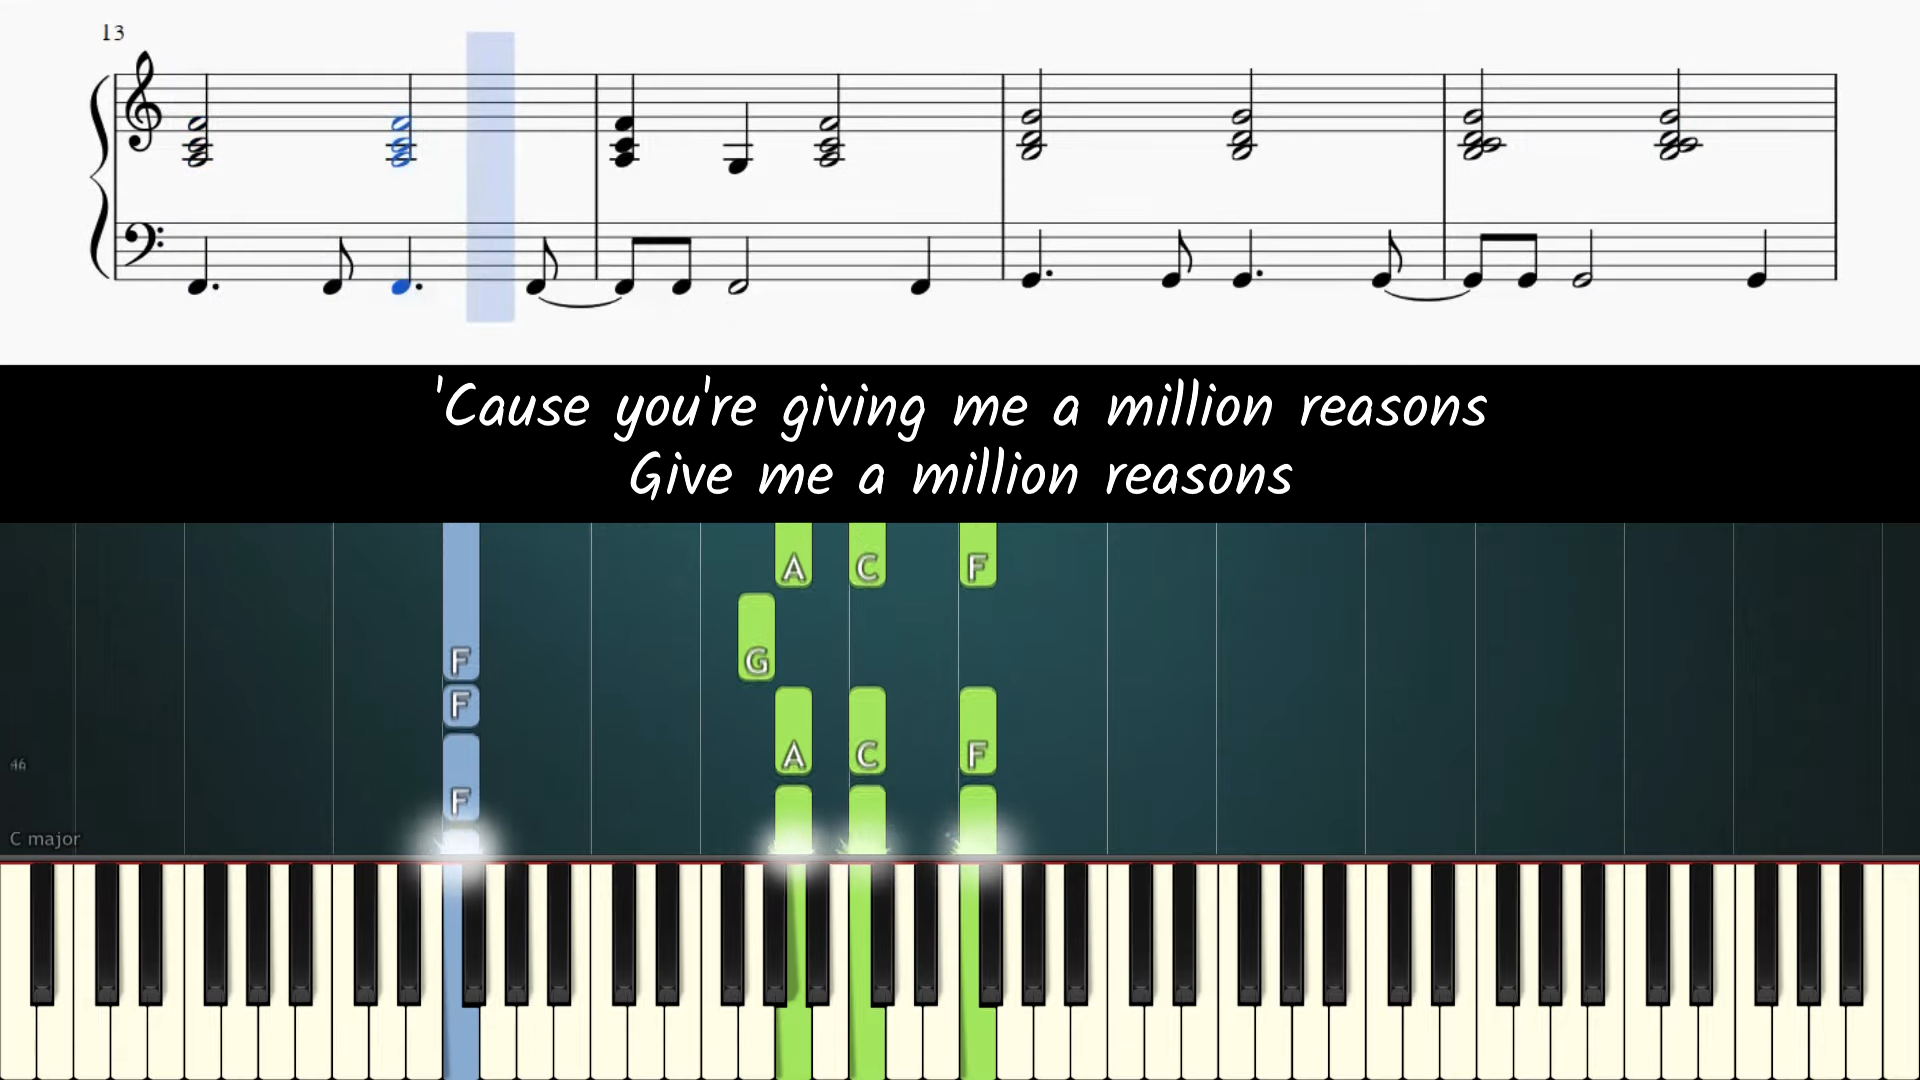
\includegraphics[scale=0.19]{milreasons.png}
	\centering
	\caption{Primjer videozapisa sa zaglavljem\cite{milreasons}}
	\label{fig:milreasons}
\end{figure}

Zbog tih razlika u dizajnu videozapisa, od korisnika se traži da na jednoj od slika iz videozapisa označi gdje se nalazi područje u kojemu se vide note (padajući pravokutnici). Pomicanjem 4 klizača, može se odrediti okvir unutar kojega se nalaze note, vidi sliku \ref{fig:screen3}. Korisnik bi trebao odabrati područje bez klavijature te po mogućnosti izostaviti dio prema klavijaturi u kojemu se prikazuju efekti kod pritiska tipke, kako bi algoritam detekcije nota preciznije radio. Na slici \ref{fig:milreasons} vide se efekti kao bijela svjetla gdje se note dodiruju s klavijaturom.

\begin{figure}[h]
	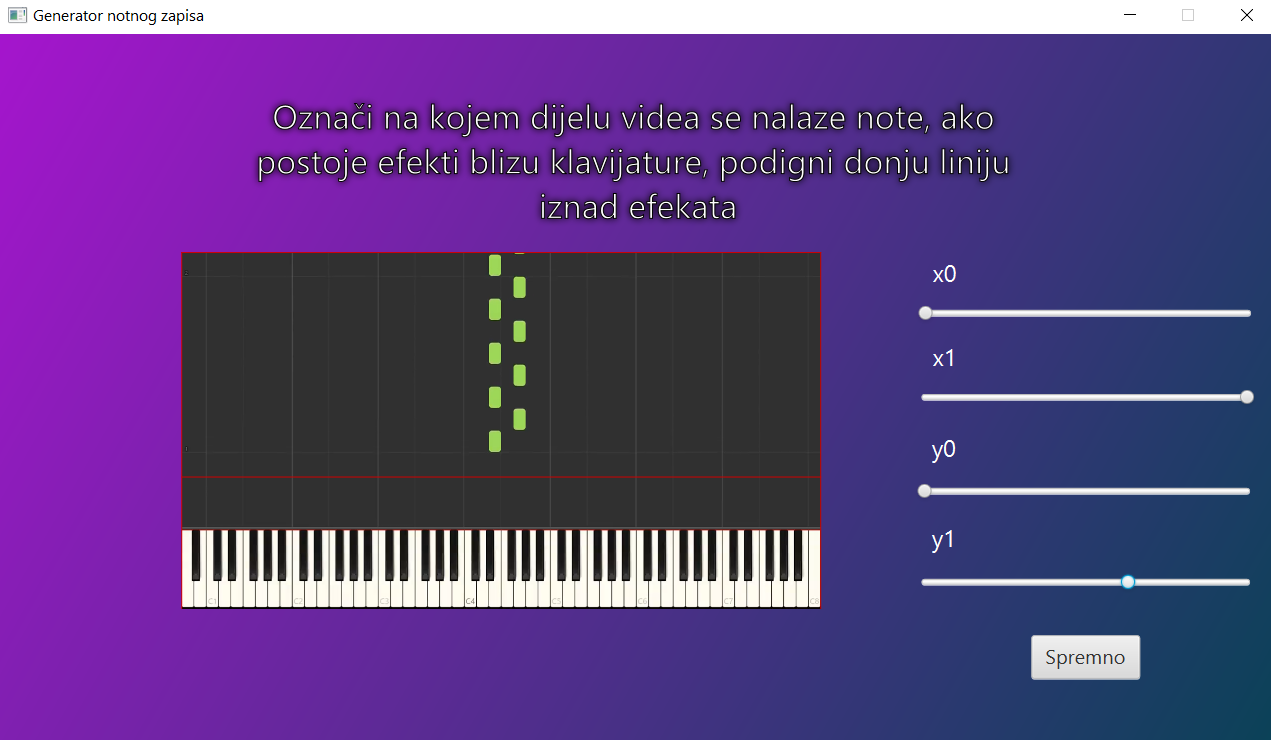
\includegraphics[scale=0.43]{screen3.png}
	\centering
	\caption{Snimka zaslona za odabir područja s notama}
	\label{fig:screen3}
\end{figure}

Nakon što je korisnik unio sve potrebno, pokreće se algoritam generiranja notnog zapisa, te se po završetku pita korisnika gdje želi spremiti generiranu datoteku.

\section{Prepoznavanje nota sa videozapisa}
Nakon izabrane klavijature i određenog područja videozapisa sa notama, pokreće se algoritam prepoznavanja nota (pravokutnika) iz slika (engl. \textit{frames}) videozapisa. Svaka se slika obrađuje, te se iz nje vade informacije potrebne za rekonstrukciju notnog zapisa. Parametri tl i br koji se šalju u metodu processFrame, označuju gornju lijevu i donju desnu točku pravokutnika koji obrubljuje područje videozapisa sa notama.

\begin{lstlisting}
VideoCapture cap = new VideoCapture(pathToVideo);
Mat originFrame = new Mat();
for(frameCounter = 1; frameCounter <
  (int)cap.get(Videoio.CAP_PROP_FRAME_COUNT); frameCounter++) {
	cap.read(originFrame);
	processFrame(tl, br, originFrame);
}
\end{lstlisting}
\subsection{Priprema slike za obradu}
Prije prikupljanja informacija o notama iz slike, treba ju se pripremiti korištenjem biblioteke OpenCV. Prvo ju se obrezuje koristeći točke pravokutnika dobivene od korisnika metodom submat.

\begin{lstlisting}
originFrame = originFrame.submat(new Rect(tl, br));
\end{lstlisting}

Zatim se provode transformacije nad slikom kako bi se dobila slika sa određenim rubovima elemenata iz kojih se mogu dobiti konture nota. Prvo se originalna slika provede kroz Gaussovo zamućivanje kako bi se smanjio šum i preciznije odredili rubovi. Zatim se slika iz BGR prostora boja (podrazumijevanog u OpenCV-u) prebaci u HSV. Iz slike u HSV formatu se uzme samo V kanal (svjetlina) te se na njega primjeni Cannyev algoritam detekcije rubova.\\

Isprobavala sam puno kombinacija prethodno navedenih koraka, te primjene Cannyevog algoritma i na H, S i V kanalu, kao i na slici s tonovima sive boje (engl. \textit{grayscale}). Također sam mijenjala i parametre metoda, međutim najbolje rezultate dobila sam upravo prikazanom kombinacijom.

\begin{lstlisting}
Imgproc.GaussianBlur(originFrame, originFrame, new Size(3, 3), 5);
Imgproc.cvtColor(originFrame, originFrame, Imgproc.COLOR_BGR2HSV);
List<Mat> hsv = new LinkedList<>();
Core.split(originFrame, hsv);
Imgproc.Canny(hsv.get(2), processedFrame, 80, 250, 3, false);
\end{lstlisting}

\subsection{Dobivanje pravokutnika iz kojih se stvaraju note}
Jednom kada je slika spremna, iz nje se mogu dobiti konture, pa iz njih pravokutnici koji predstavljaju note. Argumenti u funkciji findContours su slika iz koje se vade konture, lista u koju se žele spremiti konture, hijerarhija kontura (nije bitno ovdje), način dohvaćanja (ovdje tražim samo vanjske konture, tj. ako se kontura nalazi unutar pravokutnika, ona se ignorira) i metoda aproksimacije kontura (hoće li se spremati sve pronađene točke ili samo one potrebne za rekonstrukciju, u ovom slučaju uzela sam samo potrebne točke što daleko smanjuje zauzeće memorije).

\begin{lstlisting}
List<MatOfPoint> contours = new ArrayList<>();
Imgproc.findContours(processedFrame, contours, new Mat(), Imgproc.RETR_EXTERNAL, Imgproc.CHAIN_APPROX_SIMPLE);
\end{lstlisting}

Potom se za svaku dobivenu konturu pronalazi uspravan pravokutnik koji ju obrubljuje. Ako pravokutnik zadovoljava test, pohranjuje se u listu. Za pronalazak nota koristila sam ovaj test: \lstinline|r -> r.br().y > controlY && r.width > Constants.MIN_WIDTH && r.height > Constants.MIN_HEIGHT|. Osim što filtrira pravokutnike sa minimalnom širinom i visinom, prihvaća samo pravokutnike čija se y koordinata donjeg desnog kuta nalazi između kontrolne y koordinate i donjeg ruba slike. Kontrolna y koordinata nalazi se 20 piksela iznad dna slike.\\

Kontrolnu y koordinatu sam stavila na tu poziciju kako bih uspjela uhvatiti sve note od početka pjesme (kod većine ovakvih videozapisa, note se prvo pojave na sredini ekrana), a da i dalje imam ostavljen mali prozor za pogreške algoritma detekcije pravokutnika (u slučaju da se u nekoj od slika ne uspije detektirati početak/kraj pravokutnika, a on postoji, ima prozor od 3-4 slike za oporavak).

\begin{lstlisting}
Set<Rect> rects = new TreeSet<>(byY.reversed().thenComparing(byX));
for (int i = 0; i < contours.size(); i++) {
	Rect bounding = Imgproc.minAreaRect(new MatOfPoint2f(contours.get(i).toArray())).boundingRect();
	if(tester.test(bounding)) rects.add(bounding);
}
\end{lstlisting}

Na slici \ref{fig:controly} može se vidjeti ta kontrolna linija označena žutom bojom, a na slici \ref{fig:controlyrect} mogu se vidjeti kvadrati koji su zadovoljili taj zahtjev. Ovu liniju sam prikazala na slikama samo za pojašnjenje funkcioniranja, međutim u pravom algoritmu ona se ne crta. Također sam malo izrezala slike sa lijeve, desne i gornje strane kako bi se bolje vidjeli bitni dijelovi.

\begin{figure}[h]
	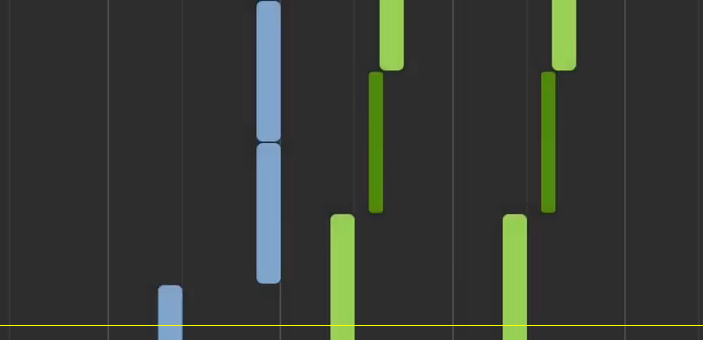
\includegraphics[scale=0.6]{controlycrop.png}
	\centering
	\caption{Primjer kontrolne linije za detekciju nota}
	\label{fig:controly}
\end{figure}

\begin{figure}[h]
	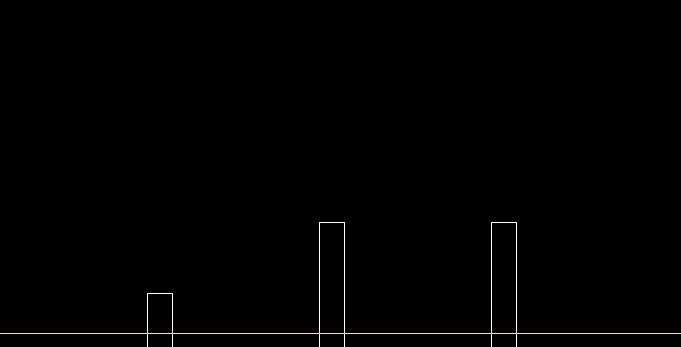
\includegraphics[scale=0.6]{controlyrectcrop.png}
	\centering
	\caption{Primjer pravokutnika koji se djelomično nalaze ispod kontrolne linije}
	\label{fig:controlyrect}
\end{figure}

Nakon pronalaska zadovoljavajućih pravokutnika, za svaki se određuje ton note (objašnjeno u nastavku). Ako se pravokutnik potpuno nalazi ispod kontrolne linije, a trenutno se ne prati nota s njegovim tonom, on se preskače jer je ili već obrađen, ili je rezultat pogreške algoritma. Nadalje, ako su u jednoj slici pronađeni pravokutnici s istim tonom, zadržava se samo onaj s većom y koordinatom (onaj koji se više "spustio"). To radim kako bih riješila eventualne pogreške u prijašnjem algoritmu (npr. ako su detektirana dva obruba oko istog pravokutnika), i pojednostavila proces detekcije trajanja nota.

\begin{lstlisting}
Map<Rect, Pitch> filtered = new TreeMap<>(byX.thenComparing(byY).reversed());
Set<Pitch> pitches = new HashSet<>();
for(Rect r : notes) {
	Pitch p = PitchConverter.getInstance().findPitch(r);
	if(r.tl().y > controlY && !currNotes.containsKey(p)) continue;
	if(!pitches.contains(p)) {
		filtered.put(r, p);
		pitches.add(p);
	}
}
\end{lstlisting}

\subsection{Određivanje tona note}
Kako bih odredila ton note (odnosno tipku kojom se svira) koristila sam sljedeći algoritam (vidi sliku \ref{fig:pitchFind} za pojašnjenje). Prvo sam odredila x koordinatu centra pravokutnika, te sam onda tome pribrojila odmak klavijature (na slici označeno OFF K narančastom bojom). Odmak je umnožak broja broj bijelih tipki koje bi se trebalo dodati prije prve da bi ona počela s \textit{c} i širine jedne bijele tipke. Npr. ako klavijatura počinje tipkom \textit{a}, onda je broj potrebnih tipki za dodati 5 (\textit{c, d, e, f, g}). Oktava se računa kao cijeli dio dijeljenja prethodno izračunatog (ljubičasto OFF C) sa širinom oktave klavijature.

\begin{lstlisting}
double keyCenter = rect.x + rect.width/2.0;
double ofsettedCenter = keyCenter + keyboard.getOffset();
int octave = (int) (ofsettedCenter/keyboard.getOctaveWidth());
\end{lstlisting}

Nakon pronalaska oktave, za određivanje tona podijelila sam ostatak prethodnog dijeljenja (na slici plavo OFF O) sa širinom tipke. Cijeli dio tog kvocijenta je broj bijele tipke u oktavi, a ostatak (na slici zeleno LO) služi kako bi se odredilo je li nota svirana crnom tipkom. Nota se smatra sniženom (svirana crnom tipkom ispred bijele) ako je ostatak manji od 20\% širine bijele tipke, a povišenom (svirana crnom tipkom nakon bijele) ako je ostatak veći od 80\%. Temeljem dobivene bijele tipke, te je li nota eventualno povišena ili snižena, može se odrediti pravi ton note uzimajući u obzir građu klavijature.

\begin{lstlisting}
double offsetInOctave = ofsettedCenter - octave*keyboard.getOctaveWidth();
int tone = (int) (offsetInOctave/keyboard.getKeyWidth());
int leftover = (int) (offsetInOctave%keyboard.getKeyWidth());

boolean isSharp = keyboard.isSharp(leftover);
boolean isFlat = keyboard.isFlat(leftover);
NoteAlphabet alphabet = switch (tone) {
	case 0 -> isSharp ? NoteAlphabet.CSH : NoteAlphabet.C;
	case 1 -> isSharp ? NoteAlphabet.DSH : (isFlat ? NoteAlphabet.CSH : NoteAlphabet.D);
	case 2 -> isFlat ? NoteAlphabet.DSH : NoteAlphabet.E;
	case 3 -> isSharp ? NoteAlphabet.FSH : NoteAlphabet.F;
	case 4 -> isSharp ? NoteAlphabet.GSH : (isFlat ? NoteAlphabet.FSH : NoteAlphabet.G);
	case 5 -> isSharp ? NoteAlphabet.ASH : (isFlat ? NoteAlphabet.GSH : NoteAlphabet.A);
	default -> isFlat ? NoteAlphabet.ASH : NoteAlphabet.H;
};
\end{lstlisting}

\begin{figure}[h]
	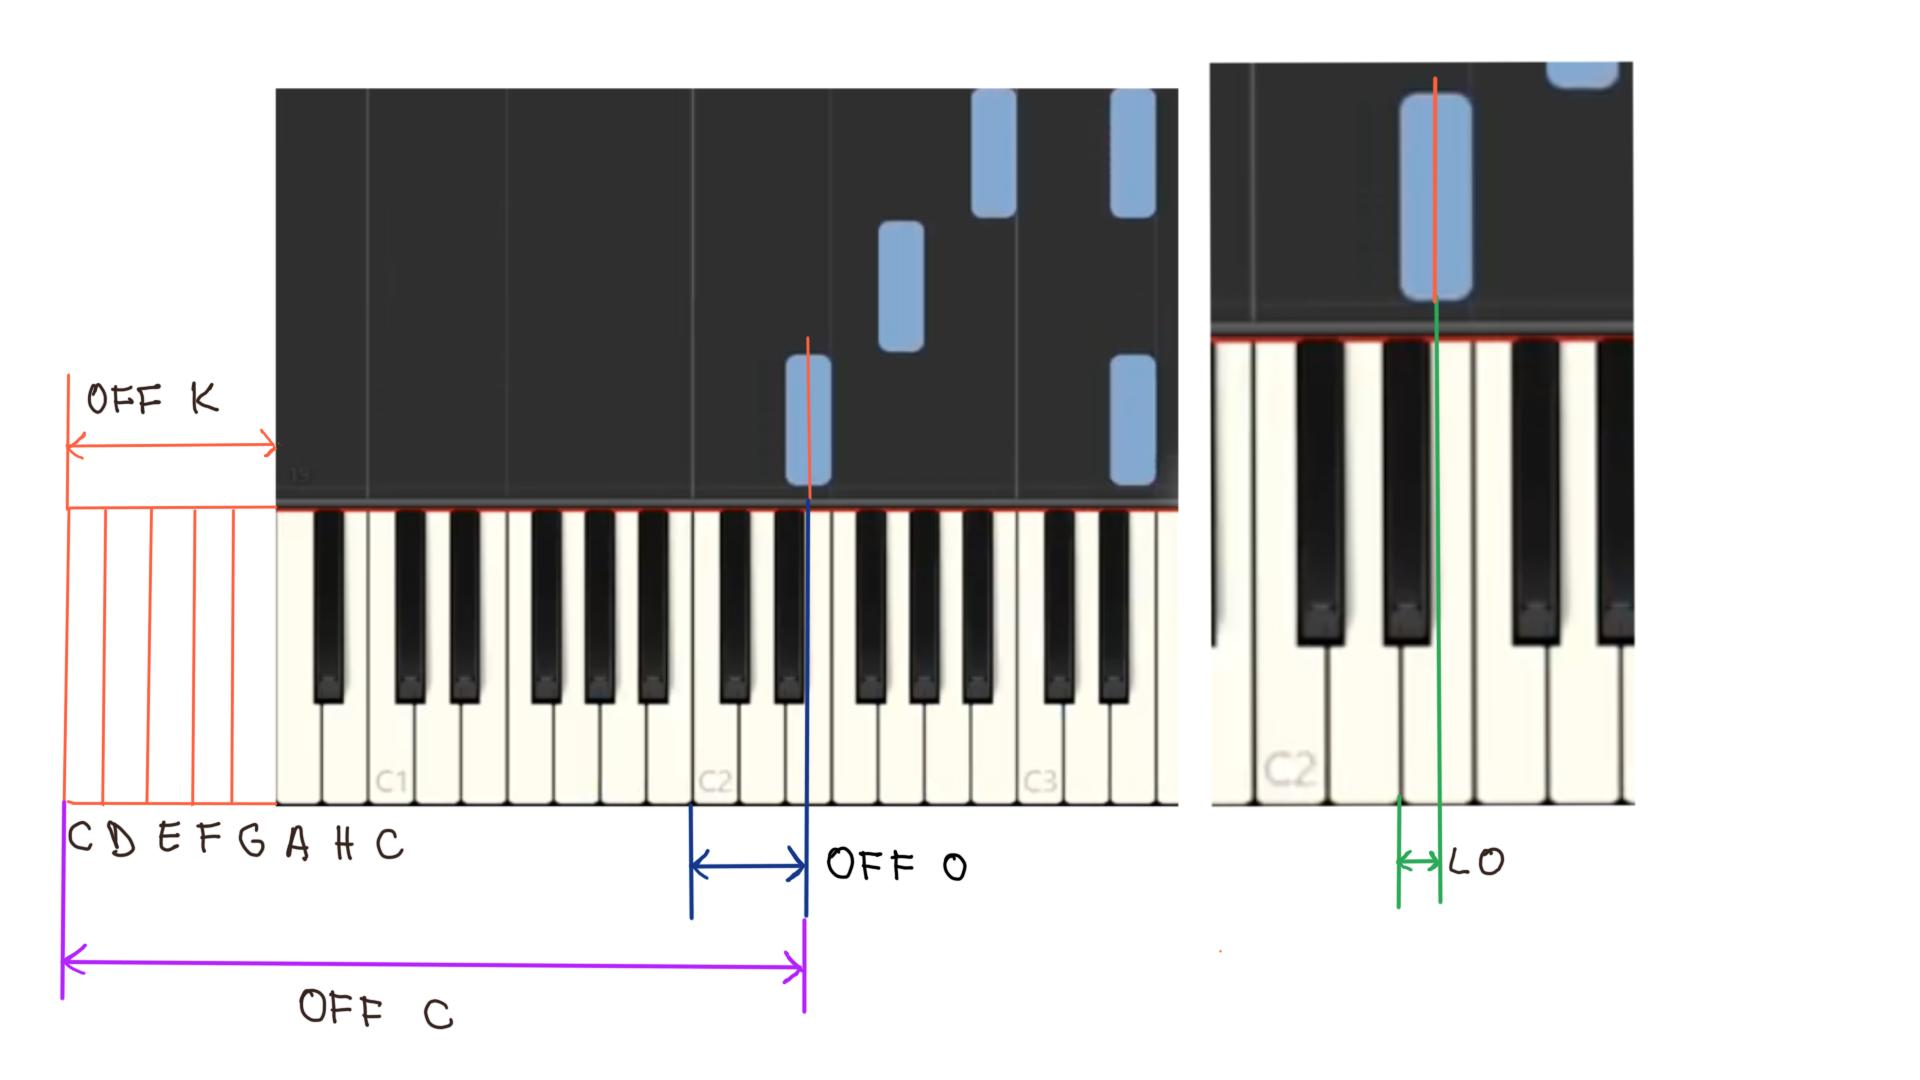
\includegraphics[scale=0.24]{pitchFind.jpg}
	\centering
	\caption{Pojašnjenje traženja tona note}
	\label{fig:pitchFind}
\end{figure}

\subsection{Pamćenje nota}
Jednom kada imam sve potrebne pravokutnike jedne slike i njihove tonove, za svaki pravokutnik radim sljedeće. Ako se u potpunosti nalazi ispod kontrolne linije, dohvaćam i brišem notu s tim tonom iz liste trenutno promatranih, postavljam joj redni broj zadnje slike u kojoj se pojavila na trenutni i dodajem ju u listu svih nota pjesme. Inače, u slučaju da se među promatranim notama ne nalazi nota s tim tonom, pronalazim kojom rukom je svirana (objašnjeno u nastavku), u trenutno promatrane dodajem novu notu s tim tonom, rukom i brojem prve slike postavljenom na trenutni i postavljam brojač egzistencije za taj ton. U slučaju da nije zadovoljen nijedan od ta dva uvjeta, znači da je nota "u prolazu", te samo resetiram brojač egzistencije.

\begin{lstlisting}
if(r.tl().y > controlY) {
	Note n = currentNotes.remove(pitch);
	currentNotesExistence.remove(pitch);
	n.setEndTime(frameCounter);
	song.addNote(n);
} else if(!currentNotes.containsKey(pitch)) {
	boolean hand = getHand(r);
	hands.get(hand).add(r.tl().x);
	currentNotesExistence.put(pitch, r.tl().y <= Constants.LONG_NOTE_TOP_Y ? Constants.EXISTENCE_LONG : Constants.EXISTENCE);
	currentNotes.put(pitch, new Note(pitch, hand, frameCounter));
} else {
	currentNotesExistence.put(pitch, r.tl().y <= Constants.LONG_NOTE_TOP_Y ? Constants.EXISTENCE_LONG : Constants.EXISTENCE);
}
\end{lstlisting}

Brojač egzistencije koristim kako bih filtrirala tonove koje algoritam detekcije krivo prepozna. U većini slučajeva kad je u pitanju pogreška, detektirani pravokutnik pojavi se u jednoj slici, te se u kasnijima više ne pojavljuje. Upravo zato kod svakog pojavljivanja tona resetiram brojač za taj ton na početnu vrijednost (4 slike). Postavila sam ju na 4 jer se nekada dogodi da pravokutnik koji postoji ne bude detektiran u nekoliko slika, pa sam time ostavila mali prozor za oporavak od pogreške. Ako se trenutni pravokutnik proteže cijelom dužinom ekrana znači da se radi o dugačkoj noti za koju je moguće da se njen pravokutnik duže vrijeme ne pojavljuje. U tom slučaju vrijeme egzistencije se postavlja na duže (200 slika). Zatim prolazim po svim brojačima i ako je neki jednak 0 znači da je vrijeme isteklo, te brišem notu s tim tonom iz liste promatranih. Inače samo smanjujem brojač za 1.

\begin{lstlisting}
for(var ex : currentNotesExistence.entrySet()) {
	if(ex.getValue() == 0) {
		currentNotes.remove(ex.getKey());
		toRemove.add(ex.getKey());
	} else ex.setValue(ex.getValue() - 1);
}
\end{lstlisting}

\subsection{Određivanje ruke kojom se svira nota}
Većina pjesama na klaviru svira se s dvije ruke (osim nekih za početnike), pa se zato na neki način note moraju razlikovati. Na videozapisu je to predstavljeno drugačijim bojama pravokutnika, što sam iskoristila da odredim kojom rukom se treba svirati koja nota. Za to sam koristila HSV verziju originalne slike. Odredila sam H (Hue) vrijednost piksela u samom centru pravokutnika na sljedeći način.

\begin{lstlisting}
double hue = originalFrame.get((int)r.tl().y + r.height/2, (int)r.tl().x + r.width/2)[0];
\end{lstlisting}

U slučaju da boja za desnu ruku još nije određena (prva nota pjesme), onda se ona postavlja na izračunatu i notu se označuje desnom rukom. Ako je određena, ali boja za lijevu ruku nije onda postoje dvije opcije: boja je dovoljno blizu desne boje (+-15) da se proglasi desnom rukom ili nije pa se lijeva boja postavlja na izračunatu i za notu se odredi da se svira lijevom rukom. U slučaju da su i jedna i druga boja određene, za notu se odredi da se svira rukom čija je boja bliža izračunatoj.\\

Na početku radim pretpostavku da će prva nota pjesme biti svirana desnom rukom, međutim to ne mora biti tako. Zbog toga pamtim x koordinate svih nota posebno za lijevu, a posebno za desnu ruku, te ako je pjesma svirana s dvije ruke (druga boja nije -1) ispravim ruke po potrebi. Računam prosjeke x koordinata lijeve i desne ruke, te sa pretpostavkom da će se note svirane lijevom rukom u prosjeku nalaziti na manjoj x koordinati nego one svirane desnom, zamijenim ruke ako to nije istina.

\begin{lstlisting}
double meanL = hands.get(true).stream().mapToDouble(d -> d).average().orElse(0.0);
double meanR = hands.get(false).stream().mapToDouble(d -> d).average().orElse(0.0);

if(meanL > meanR) song.forEach(n -> n.setLeftHand(!n.isLeftHand()));
\end{lstlisting}

\section{Prilagođavanje nota pjesmi}
Nakon što sam iz videozapisa izvukla sve informacije potrebne za izgradnju notnog zapisa, potrebno je odrediti neke parametre pjesme. Određuje se tonalitet, tempo i ritam, te se dobivene note prilagođavaju pjesmi na temelju izračunatih parametara i model pjesme se priprema za zapis u XML obliku.

\subsection{Tonalitet}
Određivanje tonaliteta pjesme nije trivijalan zadatak i ovisi o mnogo parametara, međutim uspjela sam dovoljno pojednostaviti algoritam, a da i dalje daje ispravne rezultate za veliku većinu pjesama. Osim same implementacije, puno vremena posvetila sam obnavljanju mojeg znanja teorije glazbe kako bih napisala kod u kojem nema samo hrpe hardkodiranih (engl. \textit{hardcoded}) slučajeva, nego lijepo algoritamsko rješenje koje će biti u skladu pravila teorije glazbe. Za potrebe toga napravila sam uredan API za rad sa tonovima i tonalitetima. U nastavku se mogu vidjeti neke od najvažnijih metoda, a dokumentacija i implementacija njih može se pronaći u izvornom kodu. 

\begin{lstlisting}
NoteAlphabet getSharp(NoteAlphabet n);
NoteAlphabet getFlat(NoteAlphabet n);
NoteAlphabet getMinor(NoteAlphabet n);
Set<NoteAlphabet> getSharps(int fifth);
Set<NoteAlphabet> getFlats(int fifth);
Set<NoteAlphabet> getMajorChord(NoteAlphabet n);
Set<NoteAlphabet> getMinorChord(NoteAlphabet n);
Set<NoteAlphabet> getMajorScale(NoteAlphabet n);
\end{lstlisting}

\subsubsection{Određivanje tonaliteta}
Tonalitet je sustav melodijske i harmonijske organizacije tonova skladbe oko tonike - prvog stupnja ljestvice tonaliteta. Po tonici tonalitet dobiva ime, a može biti durski ili molski\cite{tonalitet}. Tonalitet se najlakše određuje po predznacima koji se nalaze neposredno nakon ključa u notnom zapisu. Međutim, pošto mi to nije dostupno kod videozapisa, trebala sam koristiti druge metode. Algoritam koji sam napisala za otkrivanje tonaliteta dati će ispravan rezultat u većini slučajeva (znači da struktura pjesme dobro prati generalna pravila teorije glazbe), a ako ne, znači da je autor pjesme uzeo puno stilske slobode kod kompoziranja melodije.\\

Postoji 30 tonaliteta, 15 durskih i 15 molskih (točnije 24, pošto se neki preklapaju - imaju različite oznake i imena, ali isto zvuče). Tonaliteti se također dijele u kvintni (idući tonalitet u nizu je pomaknut za 5 stepeni) i kvartni krug (idući tonalitet u nizu je pomaknut za 4 stepeni), gdje pozicija u svakom krugu određuje koliko predznaka sadrži (povisilica za kvintni krug, odnosno snizilica za kvartni). Negdje se umjesto kvartnog kruga govori o tonalitetima kvintnog kruga u negativnom smjeru, pa ako se od \textit{c} ide 4 stepeni unaprijed doći će se do \textit{f}, međutim do \textit{f} se može doći i pomakom 5 stepeni unatrag. Na slici \ref{fig:fifths} može se vidjeti vizualni prikaz tonaliteta. Svaki durski tonalitet ima svoj molski komplement sa istim predznacima. \textit{C-dur}, odnosno njegov komplement \textit{a-mol} ne sadrže predznake i time su prvi tonaliteti kvartnog i kvintnog kruga.\\

\begin{figure}[h]
	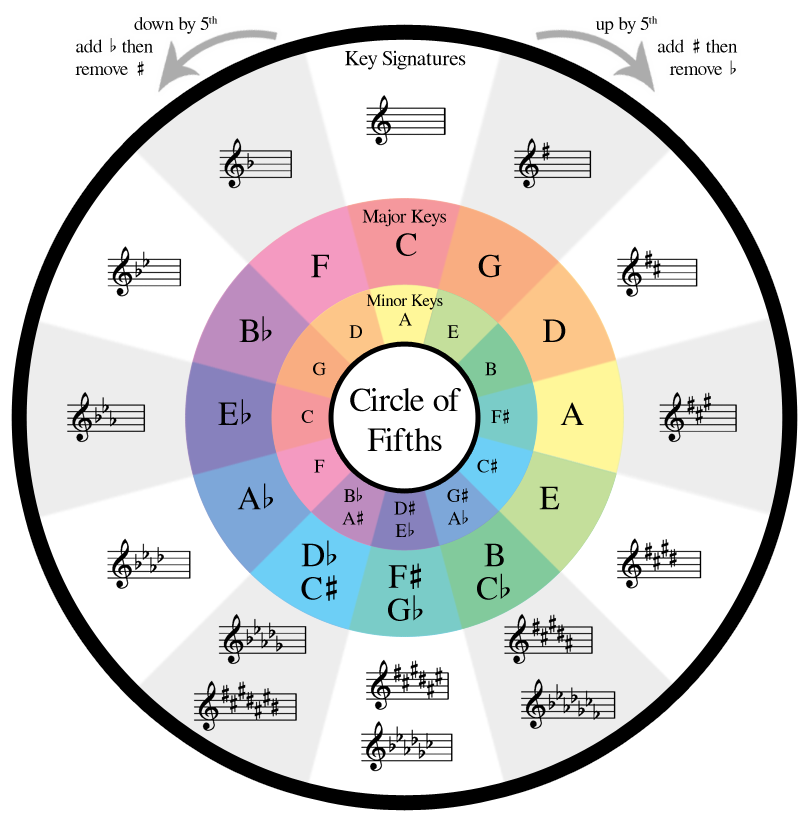
\includegraphics[scale=1.4]{fifths.png}
	\centering
	\caption{Prikaz kvintnog (i kvartnog) kruga\cite{fifths}}
	\label{fig:fifths}
\end{figure}

Kako bih odredila tonalitet pjesme, prolazila sam po svim tonalitetima, te ispitivala zadovoljava li pjesma njegove uvjete. Algoritam kreće od tonaliteta s najvećim brojem predznaka, te se usporedno ispitivajući dur i mol tonalitete, postepeno spušta prema \textit{C-duru}, tj. \textit{a-molu}. Pošto su tonaliteti koji se nalaze kasnije u krugu rjeđi i specifičniji po strukturi, dati će manje lažno pozitivnih rezultata od onih ranije, i time će algoritam imati manje pogrešaka. U slučaju da pjesma ima manje od 5 različitih tonova (pa nema dovoljno informacija), ili ne zadovolji uvjete niti jednog tonaliteta, on se postavlja na \textit{C-dur}.\\

Za potrebe algoritma određivanja pripadnosti tonalitetu, izračunala sam 5 i 10 najzastupljenijih tonova pjesme. Prvo sam odredila dur akord (odnosno mol akord ako se radi o molskom tonalitetu) ljestvice koja počinje danim tonom. To je akord koji se sastoji od 1., 3. i 5. tona u ljestvici (prima, terca i kvinta). Kod većine pjesama ta se tri tona najčešće pojavljuju što je dobar pokazatelj pripadnosti tonalitetu. U slučaju da 5 najzastupljenijih tonova sadrže sve tonove dobivenog akorda, moguće je da je pjesma tog tonaliteta, te se prelazi na drugu provjeru. Odrede se svi predznaci traženog tonaliteta (povisilice ili snizilice), te ako se u 10 nazastupljenijih tonova nalaze svi predznaci, znači da je pjesma s velikom sigurnošću tog tonaliteta.

\begin{lstlisting}
Set<NoteAlphabet> chord = isMajor ? getMajorChord(firstNote) : getMinorChord(getMinor(firstNote));
	
if(mostFreq5.containsAll(chord)) {
	Set<NoteAlphabet> alters = fifths < 0 ? getFlats(Math.abs(fifths)) : getSharps(fifths);
	if(mostFreq10.containsAll(alters))
		return new Scale(fifths, isMajor, firstNote);
}
return null;
\end{lstlisting}

\subsubsection{Prilagođavanje nota tonalitetu}
Jednom kad je tonalitet pjesme pronađen, trebaju mu se prilagoditi note. To uključuje dodavanje predznaka gdje je potrebno, te eventualno korigiranje povišenih nota u snižene i obrnuto. Npr. ako je stisnuta crna tipka između \textit{a} i \textit{h}, ton je trenutno označen kao \textit{ais (a\#)}, međutim, ako je pjesma u tonalitetu \textit{F-dur} taj ton zapravo predstavlja sniženi \textit{h (b)}. Također, tonovi nota trebaju se pripremiti za zapis u XML datoteku. Pošto MusicXML nema izravan način zapisa povišenog/sniženog tona, to se treba napraviti na malo drugačiji način. Npr. \textit{fis (F\#)} zapisuje kao \textit{f} kojemu je promjena (engl. \textit{alter}) postavljena na 1 što označava povišen ton (-1 označava snižen ton, a 0 normalan).\\

Za postizanje toga, prvo se određuju svi tonovi i predznaci ljestvice pronađenog tonaliteta. Vrijednost varijable fifths određuje poziciju tonaliteta u kvintnom krugu ako je pozitivna, odnosno kvartnom ako je negativna.

\begin{lstlisting}
int fifths = song.getScale().getFifths();
Set<NoteAlphabet> scale = getMajorScale(song.getScale().getStartAlphabet());
Set<NoteAlphabet> alters = fifths < 0 ? getFlats(-fifths) : getSharps(fifths);
\end{lstlisting}

Iteriram po svim notama pjesme, te ako je ton neke od njih snižen ili povišen u tom tonalitetu ili ako ne spada u tonalitet ali se svira crnom tipkom, treba ga izmijeniti. Ako je u pitanju kvartni krug nota je snižena, što znači da joj je promjenu potrebno postaviti na -1, a ton na pola stepena više. Npr. prepoznat je ton \textit{dis} u tonalitetu \textit{B-dur}, međutim u \textit{B-dur} ne postoji ton \textit{dis} nego \textit{es}. Povećavanjem \textit{dis} za jedan stepen dobivamo \textit{e} te ga proglašavamo sniženim. U slučaju da je prepoznati ton \textit{h} (povećavanjem dobili bi smo \textit{c}), oktava se treba povećati za jedan. Slična, samo obrnuta stvar događa se za kvintni krug. Promjena se postavlja na 1, a ton se na jedan niže. U slučaju da se radi o tonu \textit{c}, oktavu je potrebno smanjiti za 1.

\begin{lstlisting}
if(alters.contains(alph) || (!scale.contains(alph) && blackKeys.contains(alph))) {
	if(fifths < 0) {
		if(alph == NoteAlphabet.H) pitch.increaseOctave();
		pitch.setAlter(-1);
		pitch.setAlphabet(getSharp(alph));
	} else {
		if(alph == NoteAlphabet.C) pitch.decreaseOctave();
		pitch.setAlter(1);
		pitch.setAlphabet(getFlat(alph));
	}
}
\end{lstlisting}

Na kraju se još treba provjeriti nalazi li se ton u ljestvici određenog tonaliteta. Ako se ne nalazi, znači da se treba staviti predznak neposredno prije note u notnom zapisu. Predznak se određuje prema promjeni note. U slučaju da je promjena 1, dodaje se povisilica, ako je promjena -1 dodaje se snizilica a kod promjene 0 treba se staviti razrješilica koja povišeni ili sniženi ton vraća na osnovni. Pretpostavljena vrijednost promjene tona note je 0, te se ne treba eksplicitno postavljati.

\begin{lstlisting}
if(!scale.contains(alph)) note.setAccidental(pitch.getAlter());
\end{lstlisting}

\subsection{Tempo i ritam}
Nakon određivanja tonaliteta, ostalo je još odrediti tempo i ritam pjesme, te izgraditi što precizniju vremensku crtu (engl. \textit{timeline}) pojavljivanja nota i pauza. Pod pojmom tempo, ovdje mislim na broj otkucaja u minuti (engl. \textit{beats per minute}), a ritam, na mjeru pjesme. Podržani tipovi nota su: cijela nota, polovinka, četvrtinka, osminka, šesnaestinka i tridesetdruginka. Sve manje od toga ne može se precizno izračunati zbog nedovoljne preciznosti videozapisa. Jedna od korisnih mjera koju ću izračunati je broj slika po otkucaju (engl. \textit{frames per beat}), a može se jednostavnim preračunavanjem dobiti iz tempa. Označava koliko slika je trajao tip note koji je određen kao jedinica mjere.

\subsubsection{Određivanje tempa i broja slika po otkucaju}
Mjera pjesme, odnosno ritam, označuje koliko ima otkucaja (doba) u jednom taktu, i koja je jedinica mjere (koji tip note predstavlja jedan otkucaj). Tu informaciju dobijem od korisnika prije početka pokretanja algoritma procesiranja videozapisa. Od korisnika također dobijem i okvirni tempo pjesme. Kažem okvirni zato što ga koristim samo kao vodič prema ispravnom tempu. Prvo izračunam broj slika po otkucaju (\textit{fpb} u nastavku) na temelju danog tempa (\textit{bpm} u nastavku) i broja slika u sekundi koji mogu dobiti iz videozapisa (\textit{fps} u nastavku). Formula na temelju koje sam to izračunala je \textit{fpb = 60*fps/bpm}.

\begin{lstlisting}
int fps = Converter.getInstance().getFramesPerSecond();
double guessedFPB = (60.0 * fps)/song.getBeatsPerMinute();
\end{lstlisting}

Zatim odredim 5 najčešćih različitih trajanja nota (ili manje ako ih je manje od 5), te tražim koja je od tih vrijednosti najbliža izračunatoj \textit{fpb} vrijednosti. U velikoj većini pjesama jedinica mjere će se nalaziti u prvih 5 najzastupljenijih, tako da je to dovoljno dobar način određivanja. U slučaju da se dobiven \textit{fpb} razlikuje od nekog drugog unutar 5 najčešćih za 1, kao \textit{fpb} uzme se njihov prosjek. Time se osigurava da kasnije računanje bude što preciznije.\\

Tempo pjesme se ažurira na temelju izračunate \textit{fpb} vrijednosti, te se relativno trajanje takta postavlja na umnožak broja otkucaja u taktu i relativnog trajanja jedinice mjere. Relativna trajanja su harkodirana (engl. \textit{hardcoded}) te se kreću od 256 za cijelu notu, sve do 8 za tridesetdruginku. Metoda setRealDurations postavlja trajanje (u broju slika po otkucaju) svakog tipa note s obzirom na izračunato trajanje jedinice mjere (\textit{fpb}).

\begin{lstlisting}
TimeSignature ts = song.getTimeSignature();
song.setBeatsPerMinute((60 * fps)/framesPerBeat);
song.setMeasureDuration(ts.getBeats() * relativeDurations.get(ts.getBeatUnit()));
setRealDurations(framesPerBeat, ts.getBeatUnit());
\end{lstlisting}

\subsubsection{Izgradnja vremenske crte pojavljivanja nota i pauza}
Algoritam određivanja tipova nota po trajanju, te izgradnje vremenske crte pojavljivanja nota i pauza mi je bio daleko najteži problem kod izgradnje aplikacije. Zbog velike količine različitih kombinacija nota po trajanju te spajanja nota u akorde, ovaj dio aplikacije je najkompliciraniji, a i sadrži najviše mjesta za napredak i dodavanje novih funkcionalnosti.\\

Na početku algoritma odredim okvirno trajanje jednog takta pjesme i postavim početno vrijeme takta na broj slike u kojoj se prvi put pojavila neka nota. U nastavku, gdje spominjem trajanje zapravo mislim na broj slika koliko je taj element bio prisutan, a vrijeme predstavlja redni broj slike u videozapisu.
\begin{lstlisting}
double measureDuration = realDurations.get(ts.getBeatUnit()) * ts.getBeats();
\end{lstlisting}

Zatim ponavljam sljedeći algoritam sve dok ne pročitam sve note pjesme. Vrijeme kraja takta dobijem tako da zbrojim vrijeme početka i trajanje takta. U listu nota ovog takta dodam sve note za koje se u prethodnom taktu odredilo da trebaju ići u ovaj (objašnjeno u nastavku). Iteriram po notama pjesme i dodajem ih u listu nota ovoga takta dok ne naiđem na notu čije vrijeme početka nije manje od vremena kraja takta umanjenog za 2 (kako bi se ostavio prostor za pogreške). Na kraju iz liste nota pjesme izbacim sve note upravo dodane.
\begin{lstlisting}
lastMeasure = true;
List<Note> notesInMeasure = new LinkedList<>(prevMeasureNotes);
prevMeasureNotes.clear();
for(Note n : song) {
	if(!(n.getStartTime() < lastFrameOfMeasure - 2)) {
		lastMeasure = false;
		break;
	}
	notesInMeasure.add(n);
}
song.removeNotes(notesInMeasure);
\end{lstlisting}

Nakon što dobijem note takta, korigiram vrijeme završetka takta pjesme ako je potrebno. To napravim tako što pronađem najveće vrijeme završetka svih nota takta, a da je u rasponu +/-3 od prethodno izračunatog kraja takta. Ako ono ne postoji, to znači da niti jedna nota ne završava kad je kraj takta, nego ili završi ranije pa se nakon nje nalazi pauza ili se proteže u idući takt, i u tom slučaju broj se ne korigira.\\

Kako bih riješila problem nota koje se protežu kroz više taktova, obilazim sve note takta te provjeravam je li im vrijeme završetka veće od vremena kraja takta. U slučaju da je i u pitanju je zadnji takt, onda samo postavljam vrijeme kraja note na vrijeme kraja takta, inače u listu nota koje pripadaju idućem taktu dodajem notu dobivenu dijeljenjem note po vremenu kraja takta. Notu dijelim tako da napravim novu "jednaku" notu kojoj će vrijeme početka biti postavljeno na vrijeme kraja takta uvećano za jedan (početak idućeg takta), te će se na njoj postaviti kraj luka koji spaja dvije note što označava da je druga nota samo produžetak prve. Vrijeme završetka prve note se postavlja na vrijeme kraja takta i na nju se postavlja početak luka.\\

Jednom kada imam sve note takta, treba im se odrediti tip (tipovi) po trajanju. To određujem metodom koja rekurzivno traži tip note. U metodu na početku pošaljem notu za koju želim odrediti tip, jedinicu mjere kao početnu pretpostavku tipa, null kao vrijednost je li se u prethodnom pozivu tražila kraća ili duža nota i praznu listu koju se treba nadopuniti s pronađenim notama. Po završetku metode, sve pronađene note dodaju se u listu nota trenutnog takta lijeve odnosno desne ruke.\\

U slučaju da je nota unutar +/-3 duljine pretpostavljenog tipa, onda joj se tip postavlja na taj i dodaje se u listu pronađenih nota. Inače, ako je duljina kraća od pretpostavljene, a tip nije tridesetdruginka (najkraći podržani), onda postoje dva slučaja. Prvi je da je ili u prošlom pozivu rekurzije tražena kraća nota ili je ovo prvi poziv metode, te se onda poziva ista metoda ali se kao pretpostavljeni tip stavlja duplo kraći tip note, i zastavica koja označava je li se u prošlom pozivu tražila kraća nota se postavlja na \textit{true}. Drugi slučaj znači da je u prošlom pozivu tražena duža nota. To znači da se nota sastoji od više tipova i ne može joj se trajanje svesti samo na jedan. U tom slučaju nota se dijeli na dvije tako da prva traje jednako kao tip note duplo manji od pretpostavljene (najduži koji je kraći od trenutne note), a druga je ostatak. Prva se dodaje u listu pronađenih nota, a nad drugom se opet rekurzivno poziva metoda određivanja tipova. Sličan algoritam vrijedi i kada je duljina note duža od pretpostavljene, a nije cijela nota.

\begin{lstlisting}
if(realDurations.get(type) - note.getLength() > Constants.NOTE_LEN_ERROR && type != NoteType.N32TH) {
	if(prevSmaller == null || prevSmaller) {
		determineType(note, getSmaller(type), true, foundNotes);
		return;
	}
	
	Note newNote = splitNotes(note, (int) (note.getStartTime() + realDurations.get(getSmaller(type))));
	addNote(foundNotes, note, getSmaller(type));
	determineType(newNote, getSmaller(type), null, foundNotes);
} else if(note.getLength() - realDurations.get(type) > Constants.NOTE_LEN_ERROR && type != NoteType.WHOLE) {
	if(prevSmaller == null || !prevSmaller) {
		determineType(note, getBigger(type), false, foundNotes);
		return;
	}
	
	Note newNote = splitNotes(note, (int) (note.getStartTime() + realDurations.get(type)));
	addNote(foundNotes, note, type);
	determineType(newNote, getSmaller(type), null, foundNotes);
} else {
	addNote(foundNotes, note, type);
}
\end{lstlisting}

Nakon što su se svim notama odredili tipovi, vrijeme je za "izgradnju vremenske crte" što znači da se note po potrebi grupiraju u akorde i dodaju se pauze gdje je potrebno. To se radi za note svirane svakom rukom posebno. Ovaj dio algoritma je vrlo kompliciran za objasniti, jer ima puno slučajeva, pogotovo za grupiranje nota u akorde. Akord može biti "klasičan" gdje se dvije ili više nota krenu istovremeno svirati, te istovremeno završe. Međutim, postoji puno slučajeva gdje akord nije toliko "čist". Moguće je da se note krenu svirati istovremeno, pa neka od njih završi ranije, ili krenu u različito vrijeme ali završe istovremeno. Također, postoje slučajevi kada se note preklapaju pa ni ne počnu niti završe u isto vrijeme, ali se u nekom trenutku sviraju istovremeno. U tim slučajevima, pronađene note moraju se dodatno dijeliti u manje kako bi se akordi mogli ispravno prikazati. Iz tog razloga algoritam neću detaljno objašnjavati, a njegova implementacija može se pronaći u izvornom kodu.\\

Dodavanje pauza jednostavniji je dio posla. Ako obilaskom nota pronađem jednu čije je vrijeme početka za više od dvije slike nakon najkasnijeg vremena završetka prethodnih, onda se na to mjesto dodaje pauza sa trajanjem jednakim toj razlici. Nakon što su obiđene sve note takta, na sličan način dodajem pauzu na sam kraj takta ako između vremena završetka zadnje note i kraja takta postoji razlika veća od dva.

\begin{lstlisting}
if(n.getStartTime() - biggestEndFrame > Constants.REST_ERROR) {
	List<Note> foundRests = new LinkedList<>();
	Note rest = new Note(true, null, -2, false, leftHand, biggestEndFrame, n.getStartTime());
	determineType(rest, NoteType.QUARTER, null, foundRests);
	notesToAdd.addAll(foundRests);
}
biggestEndFrame = Math.max(biggestEndFrame, n.getEndTime());
\end{lstlisting}

Ovime završava algoritam građe modela pjesme, te je ona spremna za zapis u XML format datoteke.

\section{Izrada MusicXML datoteke}
Jednom kada je do kraja izgrađen model pjesme spreman za zapis u MusicXML format, težak posao je gotov. Jedino što je još preostalo je formatirati dokument na ispravan način. Da bih saznala kako treba izgledati datoteka, poslužila sam se web aplikacijom Noteflight. Napravila sam melodiju od par taktova koja je sadržavala različite vrste nota i značajke notnog zapisa kako bih vidjela na koji način se što označava u XML-u. Izvezenu datoteku u MusicXML formatu koristila sam kako bih napravila predloške (engl. \textit{template}) za izradu izlazne datoteke moje aplikacije.\\

Predloške sam koristila kako bi mi bilo lakše izgraditi MusicXML dokument. Svaki od njih predstavlja neki od elemenata dokumenta i svi su potrebni (neki i više puta) za izgradnju cijelog. Predlošci sadrže mjesta na koja se mogu ubaciti potrebne vrijednosti, a ona se označuju s dvije ljestve (\#) između kojih se nalazi ime varijable čiju je vrijednost na to mjesto potrebno upisati.\\

Na slici \ref{fig:notexml} može se vidjeti jedan od predložaka koji modelira jednu notu. Oznaka \textit{pitch} (hrv. \textit{ton}) se sastoji od tona note unutar oktave (oznaka \textit{step}), broja oktave (oznaka \textit{octave}) i mjesta na koje se može dodati oznaka \textit{alter} kojom se može sniziti ili povisiti ton u oznaci \textit{step} za 1 stepen. Oznaka \textit{duration} označava relativno trajanje note (u odnosu na trajanje takta), a \textit{type} tip note po trajanju, npr. \textit{quarter} (hrv. \textit{četvrtinka}). \textit{Staff} označava broj crtovlja u kojemu se nalazi nota, 1 za desnu ruku, a 2 za lijevu. Na mjesto označeno s \textit{\#EXT\#} mogu se dodati dodatne oznake za notu, npr. oznaka da nota spada u akord, ili da na njoj počinje ili završava luk.

\begin{figure}[h]
	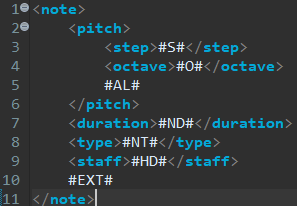
\includegraphics[scale=1.2]{notexml.png}
	\centering
	\caption{Predložak za jednu notu u MusicXML formatu}
	\label{fig:notexml}
\end{figure}

Slične predloške napravila sam i za okvir cijelog dokumenta, jedan takt, "notu" koja je pauza, te još par dodatnih. Postojanjem predložaka, građa MusicXML dokumenta svodi se na zamjenu varijabli pravim vrijednostima, te slaganjem instanci predložaka kao slagalicu. U nastavku se može vidjeti stvaranje jedne instance predloška note, te postavljanje vrijednosti varijabli. Stvara se lista taktova pjesme, te se svaki puni s ovako generiranim notama. Jednom kada su svi taktovi generirani, ugrađuju se u glavni dokument koji sadrži još neke metapodatke pjesme.

\begin{lstlisting}
String note = new String(noteTemp);

NoteAlphabet a = n.getPitch().getAlphabet();
note = note.replaceFirst("#S#", a == NoteAlphabet.H ? "B" : a.toString());
note = note.replaceFirst("#O#", String.valueOf(n.getPitch().getOctave()));
note = note.replaceFirst("#AL#", n.getPitch().getAlter() != 0
? "<alter>" + String.valueOf(n.getPitch().getAlter()) + "</alter>"
: "");

note = note.replaceFirst("#ND#", String.valueOf(n.getDuration()));
note = note.replaceFirst("#NT#", getNoteTypeString(n.getNoteType()));
note = note.replaceFirst("#HD#", n.isLeftHand() ? String.valueOf(2) : String.valueOf(1));
\end{lstlisting}

Ovime završava program.

\chapter{Analiza rezultata}
Pokretanjem aplikacije koristeći različite videozapise, uočila sam da notni zapis u izlaznoj datoteci nije uvijek 100\% jednak očekivanom. Međutim, dobiveni notni zapis je i dalje vrlo sličan željenom rezultatu, te se uz minimalne preinake korisnika, može dobiti kompletno ispravan notni zapis. U nastavku ću analizirati rezultate na pjesmi \textit{Lovely}, duet pjevačice Billie Eilish i pjevača Khalid u aranžmanu glazbenika pod imenom LittleTranscriber na YouTube-u\cite{lovely}. Odabrala sam ovu pjesmu jer se na njoj mogu jasno vidjeti dobre i loše strane moje implementacije.\\

\section{Tonalitet i tempo}
Prije nego što krenem analizirati note pjesme, reći ću nešto o rezultatima određivanja "dodatnih" podataka kao što su tonalitet i tempo pjesme. Mjeru pjesme je zadao korisnik, tako da je to očekivano ispravno prikazano u notnim zapisima svih analiziranih pjesama.\\

Kod svih pjesama koje sam testirala, tonalitet uvijek bude ispravno određen što me jako obradovalo jer nisam bila 100\% sigurna hoće li moj algoritam biti robustan po tom pitanju. Testirala sam na raznim tonalitetima kako kvintnog, tako i kvartnog kruga. Na slici \ref{fig:lovelybeg} može se vidjeti prvi takt pjesme. Nakon violinskog odnosno bas ključa, nalaze se povisilice koje određuju tonalitet. One ne mogu odrediti razliku između dur i njegovog komplementarnog mol tonaliteta, međutim to nije niti bitno za svirača. Po ovome se može zaključiti da je pjesma u \textit{G-dur} ili u \textit{e-mol} tonalitetu, a ispravan tonalitet u ovom slučaju bi bio \textit{e-mol}.\\

Tempo pjesme može se vidjeti iznad crtovlja, te mu je u ovom slučaju iznos 116 otkucaja u minuti. Nota prije tempa označava koji tip note je jedinica mjere takta, odnosno kojega tipa note je jedan otkucaj, a u ovom slučaju to je četvrtinka (što se može vidjeti i iz mjere na početku takta - četveročetvrtinska mjera). Pravi tempo ove pjesme je 115 otkucaja u minuti, no ta razlika od jednog otkucaja je zanemariva. Algoritam je robustan po pitanju tempa, jer prepozna ispravan tempo i kada korisnik unese tempo koji je relativno blizu ispravnog. Pod relativno blizu mislim da je bliži ispravnom, nego onom koji bi bio duplo brži ili duplo sporiji.

\begin{figure}[h]
	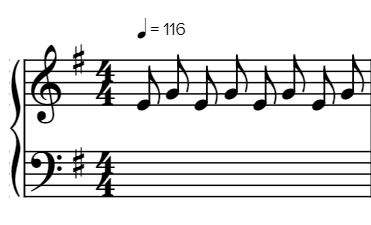
\includegraphics[scale=1]{lovelybeg.png}
	\centering
	\caption{Početak notnog zapisa pjesme \textit{Lovely}}
	\label{fig:lovelybeg}
\end{figure}

\section{Note}
Najviše grešaka kod nota događa u algoritmu prepoznavanja obrubljujućih pravokutnika. Često se dogodi da kad se ista tipka stisne dva puta zaredom (bez pauze), algoritam to prepozna kao jednu dugačku notu, međutim nekada i ispravno razlikuje dvije note. To se najčešće događa kad su u pitanju crne tipke, pošto su njihovi pravokutnici tanji i tamniji.\\

Jedan od primjera može se vidjeti na slikama \ref{fig:spojfvideo} i \ref{fig:spojfnote}. Na slici \ref{fig:spojfvideo} označeno zelenom bojom mogu se vidjeti pravokutnici koji predstavljaju note svirane desnom rukom. Dva najtamnija zelena pravokutnika označavaju notu \textit{fis}. Tipka \textit{fis} treba biti stisnuta dva puta zaredom, no može se vidjeti kako je razmak između njih malen, pa ih algoritam nekada prepozna kao jednu notu. Na slici \ref{fig:spojfnote} vidi se izgrađeni takt. Može se vidjeti kako je \textit{fis} u četvrtoj noti spojen lukom sa \textit{fisom} pete note (akorda) što označuje da je drugi \textit{fis} samo nastavak prvoga. Takve greške ne događaju se svaki puta, kao i što se može vidjeti na slikama gdje su note \textit{e} i \textit{g} uvijek ispravno razdvojene. Također, takve greške nisu "opasne" i jednostavno se isprave.\\

\begin{figure}[h]
	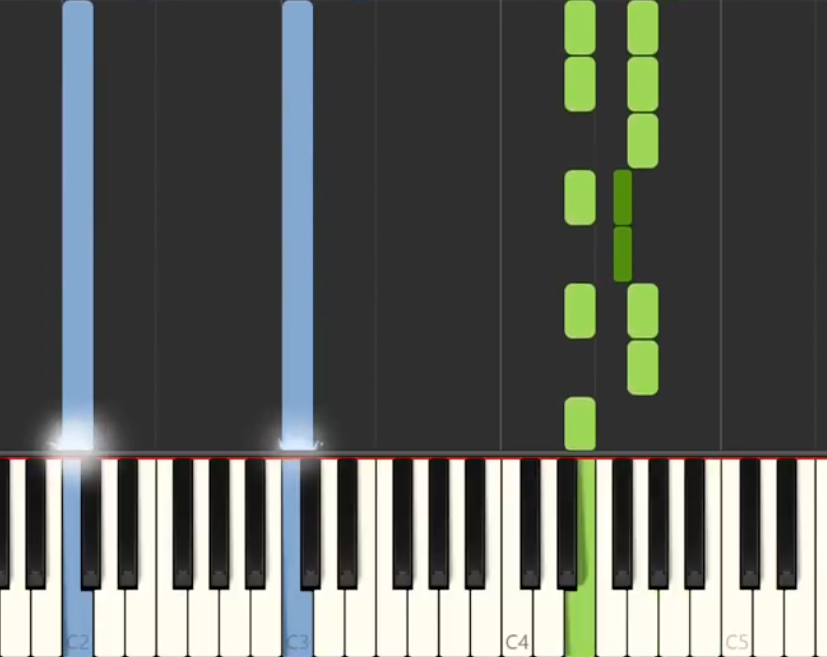
\includegraphics[scale=0.4]{spojfvideo.png}
	\centering
	\caption{Primjer istih tipki stisnutih zaredom}
	\label{fig:spojfvideo}
\end{figure}

\begin{figure}[h]
	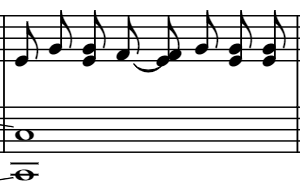
\includegraphics[scale=1]{spojfnote.png}
	\centering
	\caption{Primjer notnog zapisa krivo prepoznate note}
	\label{fig:spojfnote}
\end{figure}

Puno rjeđe zna se dogoditi da algoritam ne prepozna neku notu. Također, to se uglavnom događa s notama sviranim crnim tipkama pošto su tamnije i više se stapaju s pozadinom.\\

Ponekad se znaju događati greške u algoritmu određivanja nota po trajanju. Zbog nepreciznog algoritma detekcije nota, može se dogoditi da trajanje note bude kraće ili dulje od očekivanog. Takve greške budu neugodnije jer se poremeti ritam pjesme. Jedna takva greška može se vidjeti na slici \ref{fig:ritamerror}. Zbroj trajanja nota desne ruke je 4.25 dobe, znači da ima jedna šesnaestinka viška. Upravo zato note nisu poravnate s notama lijeve ruke. To se dogodilo iz razloga zato što je zaokružena nota proglašena osminkom, a trebala je biti šesnaestinka. Na sreću, te pogreške ne događaju se često. Također, pogreške iz jednog takta ne propagiraju se u druge, tako da ih je vrlo lagano ručno ispraviti.\\

\begin{figure}[h]
	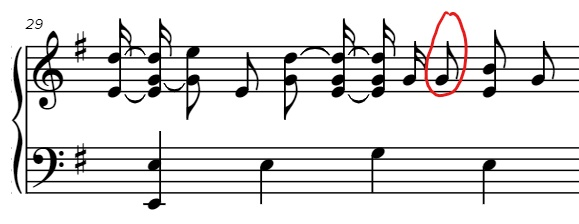
\includegraphics[scale=0.7]{ritamerror.jpg}
	\centering
	\caption{Pogreška u ritmu pjesme}
	\label{fig:ritamerror}
\end{figure}

Kod određivanja tona note nisam nijednom primjetila pogrešku, kao ni kod određivanja kojom rukom se svira koja nota. Kao što je i očekivano, većina grešaka događa se u ritmu pošto je to i bio najkompliciraniji dio aplikacije za implementirati.\\

Iako ovako zvuči kao da algoritam ima dosta pogrešaka, od 93 takta pjesme \textit{Lovely} greške (ubrajajući i one male) događaju se samo u njih 15, što je prilično dobar rezultat. Još jedan pokazatelj kvalitete može se vidjeti na slici \ref{fig:super}. Prepoznate su note od onih najđužih (dupla cijela nota u lijevoj ruci) do skoro najkraćih (šesnaestinke u desnoj ruci).

\begin{figure}[h]
	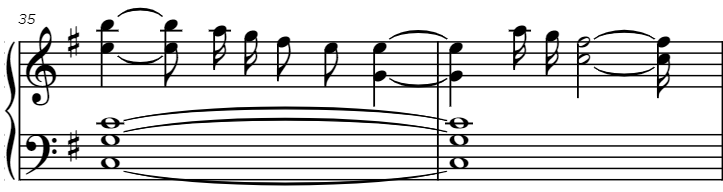
\includegraphics[scale=0.75]{super.png}
	\centering
	\caption{Primjer dobrog prepoznavanja}
	\label{fig:super}
\end{figure}

\chapter{Zaključak}
Radeći ovaj rad, shvatila sam koliko je težak zadatak povezati nešto subjektivno kao što je glazba, s računalom koje traži pravila i determinizam. Mnoge stvari koji ljudi uzimaju "zdravo za gotovo", računalu je vrlo teško. Ljudsko oko i mozak otporni su na manje greške, te razumiju značenje kroz kontekst, dok računalo ne može "razmišljati" na taj način, pa je u mnogim algoritmima potrebno uzimati u obzir manje anomalije kako bi se mogao dobiti ispravan rezultat.\\

Glazba ima ogromnu količinu pravila, ali zato još i više iznimki. Također, često ostavlja veliki prostor glazbenicima za izražavanje svoje kreativnosti i stila, te ju je upravo iz tog razloga vrlo teško strukturirati na oblik razumljiv računalu.\\

U ovom radu nisam obradila niti polovicu "funkcionalnosti" koje glazba pruža, jer ih ima jako puno, a velika količina njih niti nije čitljiva kroz videozapise koje sam obrađivala. Pravi notni zapis, kojega je radio iskusni glazbenik/skladatelj, nudi veliki broj dodatnih oznaka koje obogaćuju glazbu. Od razlika u tempu i dinamici (glasnoći izvođenja određenih dijelova), do načinu izvođenja nota (npr. \textit{staccato} ili \textit{legato}), pa do korištenja pedala klavira (jedna služi za stišavanje note, druga za produžetak trajanja i nakon što se tipka otpusti). Iz tog razloga mislim da nikakva aplikacija ili videozapisi neće moći zamijeniti pravi notni zapis, međutim za potrebe zabave i brzog učenja ovo je vrlo korisno.\\

Iako moja aplikacija ne daje 100\% točne rezultate, i dalje mislim da je vrlo korisna i ima svoju namjenu. Dok sam aktivno svirala klavir, prije 7-8 godina, bila bih oduševljena ovakvom aplikacijom jer bi mi uvelike ubrzala proces svladavanja pjesme koju sam htjela naučiti iz takvih videozapisa. Vrijeme koje bih potrošila za napraviti minimalne izmjene u dobivenom notnom zapisu bilo bi zanemarivo prema vremenu i trudu koje sam inače ulagala kako bih ručno iz videozapisa dobila notni. Upravo zbog toga sam vrlo ponosna na svoj konačan proizvod.

\bibliography{literatura}
\bibliographystyle{fer}

\begin{sazetak}
U ovom radu proučavala sam problem generiranja notnog zapisa iz videozapisa koji padajućim linijama prikazuje u kojem trenutku je pritisnuta koja tipka klavijature. Analiziranjem svake slike videozapisa, dobivala sam informacije o pritisnutim tipkama, te sam ih koristila kako bih izgradila model pjesme. Korištenje aplikacije vrlo je jednostavno: korisnik odabere željeni videozapis, zada određene parametre pjesme (npr. raspon klavijature, mjera i okvirni tempo pjesme), i kao izlaz dobije datoteku u MusicXML formatu koja sadrži sve bitne informacije za generiranje notnog zapisa. Učitavanjem dobivene datoteke na jedan od mnogih alata dostupnih na Internetu, korisnik može dobiti notni zapis u PDF obliku. Zbog širokih mogućnosti glazbe, i slobode glazbenika, kod implementacije programa suočavala sam se s mnogim naizgled trivijalnim ali vrlo kompleksnim problemima. Korisnost ovog programa je vrlo velika čak i ako ne daje 100\% točne rezultate, jer na sebe preuzima ogromnu količinu posla, a za glazbenika ostavlja samo male korekcije. U radu je objašnjena implementacija programskog rješenja, te su navedeni i analizirani dobiveni rezultati.

\kljucnerijeci{generiranje notnog zapisa, glazba, računalni vid, detekcija objekata, obrada slike, obrada videozapisa}
\end{sazetak}

\pagebreak

\engtitle{Music score generation from video stream of piano keyboard time traces}
\begin{abstract}
In this paper, I studied the problem of generating sheet music from a video that uses falling lines to show at what time which key on the piano keyboard was pressed. By analyzing each frame of the video, I received information about the keys pressed, and used it to build a song model. Using the application is very simple: the user selects the desired video, sets certain parameters of the song (e.g.piano  keyboard range, measure and approximate tempo of the song), and as an output receives a file in MusicXML format that contains all the important information to generate the sheet music. By uploading the resulting file to one of the many tools available on the Internet, the user can get the sheet music in PDF format. Due to the wide possibilities of music, and the freedom of musicians, I faced many seemingly trivial but very complex problems when implementing the program. The usefulness of this program is large even if it does not give 100\% accurate results, because it takes on a huge amount of work, and leaves the musician to deal with only small corrections. The implementation of the software solution is explained in this paper, and the obtained results are listed and analyzed.

\keywords{sheet music generation, music, computer vision, object detection, image processing, video processing}
\end{abstract}

\end{document}
